\documentclass[10pt,letterpaper,twoside]{article}

\usepackage{gensymb}
\usepackage[labelformat=simple]{subcaption}
\renewcommand*{\thesubfigure}{\Alph{subfigure}}
\usepackage{tabularx, multirow}
\usepackage{makecell}
\usepackage{hyperref}
\hypersetup{draft}

\renewcommand{\figurename}{Fig}

\usepackage{siunitx}
\sisetup{output-exponent-marker=\ensuremath{\mathrm{e}}}

\bibliographystyle{plos2015}

\usepackage{threeparttable}
\usepackage[dvipsnames]{xcolor}
%\usepackage{enumitem}
%\newcommand{\method}[1]{\qquad Method #1}
\usepackage{graphicx}
\usepackage{soul}
\usepackage{xspace}
\usepackage[margin=1in]{geometry}
\newcommand{\indep}{\rotatebox[origin=c]{90}{$\models$}}
\newcommand{\eg}{\emph{e.g.}\xspace}
\newcommand{\ie}{\emph{i.e.}\xspace}
\newcommand{\T}{^\mathrm{T}}
\newcommand{\bbeta}{\boldsymbol{\beta}}
\newcommand{\blup}{\widetilde{\bbeta}}
\newcommand{\bzero}{\mathbf{0}}
\newcommand{\bI}{\mathbf{I}}
\newcommand{\bx}{\mathbf{x}}
\newcommand{\bX}{\mathbf{X}}
\newcommand{\by}{\mathbf{y}}
\newcommand{\tausq}{\tau^{2}}
\newcommand{\qtl}{\widehat{h^{2}}_{\text{QTL}}}

%\newlength{\myFootnoteLabel}
%\newenvironment{tableminipage}[1]{\begin{minipage}{#1}\renewcommand\footnoterule{ \kern -1ex}%
%\setlength{\myFootnoteLabel}{0.5em}%
%}{\end{minipage}}

\newcommand{\permpc}{\text{permP}_{\text{C}}}
\newcommand{\permpg}{\text{permP}_{\text{G}}}

\newcommand{\permpmed}{\text{permP}^{m}}

\newcommand{\ctwohtwo}{\texorpdfstring{C\textsubscript{2}H\textsubscript{2}}}

\begin{document}

\section*{S1 Appendix: CC strains}

This study included males from the following 47 CC strains: CC001, CC002, CC003, CC004, CC005, CC006, CC007, CC010, CC011, CC012, CC013, CC015, CC016, CC017, CC019, CC020, CC021, CC023, CC024, CC025, CC027, CC028, CC029, CC030, CC031, CC032, CC033, CC035, CC036, CC037, CC038, CC039, CC040, CC041, CC042, CC043, CC044, CC045, CC046, CC049, CC053, CC055, CC057, CC059, CC061, CC062, and CC068.

\newpage

\section*{S2 Appendix: Detailed description of conditional genome-wide scans}

Combining a per-trait family-wise error rate (FWER) control and across-trait false discovery rate (FDR) control restricts the mapping procedures ability to detect multiple QTL per outcome in a fully valid manner because the generalized extreme value distribution (GEV) used for FWER control is fit from the maximum statistical score per trait. To include additional strong statistical scores is potentially biasing, as would be the case when there are multiple associations above the FWER threshold, increasing the enrichment in small $p$-values. This inflation is precisely the pattern of association the FDR procedure detects. To avoid this problem, a multi-stage conditional regression approach was used \cite{Jansen2017}. The procedure is described in the following steps:
\begin{enumerate}
    \item For a given trait, conduct a genome scan according to this model: 
\begin{equation}
    y_i = \mu + \text{batch}_{b[i]} + \text{QTL}_i + \varepsilon_i,
      \label{eq:alternative_model}
 \end{equation}
    where $y_{i}$ is the trait level for individual $i$, $\mu$ is the intercept, $\text{batch}_b$ is a categorical fixed effect covariate with five levels $b=1,\dots,5$ representing five sequencing batches for both gene expression and chromatin accessibility and $b[i]$ denoting the batch relevant to $i$, $\varepsilon_i\sim\text{N}(0,\sigma^2)$ models the residual error, and $\text{QTL}_{i}$ models the genetic effect at the locus.
    \item Perform genome scans for the permuted trait to characterize a GEV. Calculate a genome-wide error rate controlled $p$-value, $\permpg$, from the observed maximum logP of the genome scan of the trait. The $\permpg$ is stored to be used as input to an FDR procedure.
    \item Specify a genome-wide $\alpha_{\text{step}}$ for determining whether subsequent conditional scans should be conducted for the trait. We set $\alpha_{\text{step}} = 0.1$. If $\permpg > \alpha_{\text{step}}$, no further conditional scans are conducted.
    \item If $\permpg \le \alpha_{\text{step}}$, steps 1-3 are repeated for an additional conditional scan of the outcome. For $j > 1$, the $j^{\text{th}}$ conditional scan uses the same form of alternative and null model as described in Eq \ref{eq:alternative_model}, except with the inclusion of locus effects from the peak associations from previous stages. Generally, the alternative model for conditional scan $J$ follows as:
\begin{equation}
y_{i} = \mu + \text{QTL}_{i} + \sum_{j=1}^{J-1}\text{locus}_{i}^{j} + \text{batch}_{b[i]} + \varepsilon_{i},
\label{eq:conditional_model}
\end{equation}
with $\text{locus}_{i}^{j}$ representing the locus effect of the peak association from the $j^{\text{th}}$ stage scan of the outcome for individual $i$, and is also included in the null model of conditional scans. Now steps 2-4 are repeated.
\end{enumerate}

A multi-stage conditional scan approach could have issues with over-fitting 47 data points per trait, given that each $\text{QTL}$ and $\text{locus}$ effect represents the estimation of seven fixed effects. However, the permutations were found to appropriately compensate for this potential problem in the recalculation of the GEV based on permutations of the conditional scans in step 2. S21 Fig provides a clear example in which the gene \textit{Gpn3} has a local-eQTL detected after a strong distal-eQTL is conditioned for within the model in lung tissue. 

\newpage

\section*{S3 Appendix: Mediation analysis}

For this study, simple models that consist of three variables are used: the independent variable X, the mediator M, and the dependent variable Y \cite{Baron1986,MacKinnon2007}. Superscripts are used to indicate whether a variable is the QTL, chromatin accessibility at site $k$ ($\text{C}_{k}$), or expression of gene $j$ ($\text{G}_{j}$) in the model. When an eQTL is detected, the following relationship is supported:
\begin{equation}
\text{X}\textsuperscript{QTL} \quad \rightarrow \quad \text{Y}^{\text{G}_{j}}
\label{rel:eQTL}
\end{equation}
When cQTL or proximal eQTL to distal-eQTL are detected, a similar relationship is detected:
\begin{equation}
\text{X}\textsuperscript{QTL} \quad \rightarrow \quad \text{M}
\label{rel:cQTL}
\end{equation}
The previous traits (Y) can also be viewed as potential mediators (M). Here we consider two models of mediation: 1) the effect of an eQTL is mediated through local chromatin state ($\text{M}^{C_{k}}$) and 2) the effect of the distal-eQTL is mediated through a proximal gene ($\text{M}^{G_{k}}$), depicted in Fig 6. Co-localizing QTL are consistent with the co-occurrence of $X \rightarrow Y^{G_{j}}$ and $X \rightarrow Y^{C_{k}}$ at a locus. A true mediation relationship has an additional requirement, specifically that: 
\begin{equation}
\text{X}\textsuperscript{QTL} \quad \indep \quad \text{Y}^{\text{G}_{j}} \quad | \quad \text{M}
\label{rel:full_mediator}
\end{equation}
where ``A $\indep$ B'' indicates that A and B are independent of each other, and ``A $|$ B'' is A conditioned on variable B. X being fully independent of Y given M is consistent with X acting on Y completely through M, referred to as full mediation. In practice, the true relationship can be complex and obscured by noise, instead resulting in partial mediation, whereby X affects Y both directly and through M. Genome-wide data present a significant challenge to systematically testing these relationships.

\subsection*{Mediation permutation scans}

Empirical $p$-values for the mediators can be defined through permutations, similarly to as is done with the QTL. Instead of permuting the trait outcome, the pairing of trait to QTL is maintained, and the mediator is permuted. GEVs are then fit for potential mediators from the minimum logP from the permutation scans, instead of the maximum logP in QTL scans. FWER-controlled mediation $p$-values are calculated from the GEV: $\permpmed = F_{\text{GEV}}(\text{logP})$. An FDR adjustment is not used with mediation because it is only evaluated for detected QTL, which violates the uniform null distribution expectations of FDR.

\subsection*{Mediation models}

\subsubsection*{Mediation of local-eQTL through chromatin state.}
Mediation through chromatin accessibility was evaluated for all local-eQTL detected through the lenient Analysis L, leveraging prior knowledge of the predominance of local genetic regulation and the effects of proximal chromatin state. Candidate mediators are detected at genome and chromosome-wide significance through 1,000 permutations to define GEVs for FWER control of minimum mediation logP. Genome-wide mediation is detected if $\permpmed_{\text{G}} < 0.05$ and local chromosome-wide if $\permpmed_{\text{C}} < 0.05$. 

\subsubsection*{Mediation of distal-eQTL through local gene expression.}
Mediation of the effect of genome-wide significant distal-eQTL through proximal gene expression was evaluated. Genome-wide significance is required for distal-eQTL because there is not additional strong biological information to support reduced stringency as is the case with local signal. As with mediation through chromatin state, 1,000 permutations are used to define genome-wide mediation $p$-values, $\permpmed_{\text{G}}$. 

Mediation of cQTL through other chromatin sites and gene expression were also considered, but did not result in the detection of any candidate mediators.

\subsection*{Formal mediation criterion}

Detection of mediation has some caveats and pitfalls compared to the statistical analyses used for QTL mapping, in part due to the fact that the relationships \ref{rel:eQTL} and \ref{rel:cQTL} could be complex, whereas the directionality of the relationships for QTL is fixed because the genetic state at the QTL cannot change because of the trait. This does not hold for the mediation model, where Y could in fact causally influence M (Y $\rightarrow$ M). \cite{Didelez2007} note that false mediation signals can be detected when the association between the M and Y are particularly strong, whereby M acts as a surrogate for X. Based on concerns over fitting relatively complex models to data comprising 47 observations, we use stringent requirements for declaring evidence for mediation:
\begin{enumerate}
	\item Detection of a significant eQTL (relationship \ref{rel:eQTL}).
    \begin{enumerate}
    	\item Mediation through chromatin: $\permpmed_{\text{C}} < 0.05$ from Analysis L
        \item Mediation through expression: $\permpmed_{\text{G}} < 0.05$ from Analysis G
    \end{enumerate}
    \item Detection of significant mediator within a 20Mb window centered around the eQTL from previous step.
    \item Detection of a significant QTL for the mediator from previous step.
    \begin{enumerate}
    	\item Mediation through chromatin: $\permpmed_{\text{C}} < 0.05$ from Analysis L and within 10Mb upstream or downstream of gene TSS
        \item Mediation through expression: $\permpmed_{\text{G}} < 0.05$ from Analysis G and within 10Mb upstream or downstream of the eQTL position
    \end{enumerate}
    \item It is not possible to distinguish M $\rightarrow$ Y from M $\leftarrow$ Y given these data. If M is an intermediary of X on Y, the expectation is that the effect of X $\rightarrow$ M is greater than X $\rightarrow$ Y. We check that the effect size of the QTL for step 1 (X $\rightarrow$ Y) is less than the effect size of the QTL from step 3 (X $\rightarrow$ M). Failure of this step does not disprove the proposed mediation model, but it could suggest that the relationship between M and Y is more complicated than the simple models tested here, or that greater noise is incurred in the measurement of M than Y.
\end{enumerate}

\newpage

\begin{thebibliography}{10}

\bibitem{Jansen2017}
Jansen R, Hottenga JJ, Nivard MG, Abdellaoui A, Laport B, de~Geus EJ, et~al.
\newblock {Conditional eQTL analysis reveals allelic heterogeneity of gene
  expression.}
\newblock Human Molecular Genetics. 2017;26(8):1444--1451.
\newblock doi:{10.1093/hmg/ddx043}.

\bibitem{Baron1986}
Baron RM, Kenny DA.
\newblock {The moderator-mediator variable distinction in social psychological
  research: Conceptual, strategic, and statistical considerations.}
\newblock Journal of Personality and Social Psychology. 1986;51(6):1173--1182.
\newblock doi:{10.1037/0022-3514.51.6.1173}.

\bibitem{MacKinnon2007}
MacKinnon DP, Fairchild AJ, Fritz MS.
\newblock {Mediation Analysis}.
\newblock Annual Review of Psychology. 2007;58(1):593--614.
\newblock doi:{10.1146/annurev.psych.58.110405.085542}.

\bibitem{Didelez2007}
Didelez V, Sheehan N.
\newblock {Mendelian randomization as an instrumental variable approach to
  causal inference.}
\newblock Statistical Methods in Medical Research. 2007;16(4):309--30.
\newblock doi:{10.1177/0962280206077743}.

\bibitem{HamiltonWilliams2013}
Hamilton-Williams EE, Rainbow DB, Cheung J, Christensen M, Lyons PA, Peterson
  LB, et~al.
\newblock {Fine mapping of type 1 diabetes regions Idd9.1 and Idd9.2 reveals
  genetic complexity.}
\newblock Mammalian Genome. 2013;24(9-10):358--75.
\newblock doi:{10.1007/s00335-013-9466-y}.

\end{thebibliography}

\newpage

\section*{Supplemental tables and figures for Keele \& Quach \textit{et al.}}

%%%%%%%%%% Supplement
\setcounter{table}{0}
\setcounter{figure}{0}
\renewcommand{\thetable}{S\arabic{table}}
\renewcommand{\thefigure}{S\arabic{figure}}
\setcounter{page}{1}

\begin{table}[h]
\centering
\begin{threeparttable}[b]
\caption{\bf Number of differentially expressed genes and accessible chromatin regions detected between liver, lung, and kidney tissues at FDR $<$ 0.1
\label{tab:diff_gene}}
\begin{tabularx}{\textwidth}{ll|XXX}
\hline 
& & & \center{Tissue comparison} & \\
& & Liver/lung & Liver/kidney & Lung/kidney \\
\hline
%%%%%%%%%%%%%%%%
Genes & Up-regulated & 2,473 (20.8\tnote{a}) & 2,123 (17.9\tnote{a}) & 2,246 (18.9\tnote{a}) \\
& Down-regulated & 3,236 (27.2\tnote{a}) & 1,441 (12.1\tnote{a}) & 2,527 (21.3\tnote{a}) \\
& Total & 5,709 (48.0\tnote{a}) & 3,564 (30.0\tnote{a}) & 4,773 (40.2\tnote{a}) \\
\cline{2-5}
Chromatin regions & Increased accessibility & 20,194 (19.6\tnote{b}) & 15,252 (12.9\tnote{b}) & 19,202 (17.4\tnote{b}) \\
& Decreased accessibility & 20,603 (19.7\tnote{b}) & 12,796 (11.4\tnote{b}) & 12,967 (11.2\tnote{b}) \\
& Total & 40,797 (39.3\tnote{b}) & 28,048 (24.3\tnote{b}) & 32,169 (28.6\tnote{b}) \\
\hline
\end{tabularx}
\begin{tablenotes}
     \item[a] Percentage of all tested genes.
     \item[b] Percentage of all tested chromatin regions prior to merging adjacent genomic windows.
   \end{tablenotes}
\end{threeparttable}
\end{table}


\begin{table}[h]
\centering
\begin{threeparttable}[b]
\caption{\bf Number of genes with eQTL detected in liver, lung, and kidney tissues at FDR $<$ 0.1
\label{tab:eqtl_mapping}}
\begin{tabularx}{\textwidth}{ll|XXX}
\hline 
& & & \center{Tissue (\%)} & \\
Procedure & eQTL type & Liver & Lung & Kidney \\
\hline
%%%%%%%%%%%%%%%%
Analysis G & All & 520 (6.2\tnote{a}) & 478 (4.2\tnote{a}) & 739 (7.3\tnote{a}) \\
& Local\tnote{d} & 400 (76.9\tnote{b}) & 369 (77.2\tnote{b}) & 601 (81.3\tnote{b}) \\
& Distal\tnote{e} & 132 (25.4\tnote{b}) & 112 (23.4\tnote{b}) & 148 (20.0\tnote{b}) \\
\hline
% %%%%%%%%%%%%%%%%
Analysis C & All & 2,587 (30.8\tnote{a}) & 2,069 (18.2\tnote{a}) & 3,191 (31.6\tnote{a}) \\
& Local\tnote{d} & 1,749 (67.6\tnote{c}) & 1,498 (72.4\tnote{c}) & 2,214 (69.4\tnote{c}) \\
& Distal\tnote{e} & 838 (32.4\tnote{c}) & 571 (27.6\tnote{c}) & 977 (30.6\tnote{c}) \\
\hline
% %%%%%%%%%%%%%%%%
Analysis L\tnote{f} & Genome-wide FWER $<$ 0.05 & 702 (8.4\tnote{a}) & 713 (6.3\tnote{a}) & 955 (9.5\tnote{a}) \\
& Chromosome-wide FWER $<$ 0.05 & 1,661 (19.8\tnote{a}) & 1,880 (16.6\tnote{a}) & 2,102 (20.8\tnote{a}) \\
\hline
\end{tabularx}
\begin{tablenotes}
     \item[a] Percentage of all tested genes.
     \item[b] Percentage of genes with eQTL from Analysis G.
     \item[c] Percentage of genes with eQTL from Analysis C.
     \item[d] Within 10Mb upstream or downstream of gene TSS.
     \item[e] More than 10Mb upstream or downstream of gene TSS, or on another chromosome.
     \item[f] Not FDR controlled.
   \end{tablenotes}
\end{threeparttable}
\end{table}

\clearpage

\begin{table}[h]
\centering
\begin{threeparttable}[b]
\caption{\bf Number of genes with eQTL detected in liver, lung, and kidney tissues at FDR $<$ 0.2
\label{tab:eqtl_mapping_lenient}}
\begin{tabularx}{\textwidth}{ll|XXX}
\hline 
& & & \center{Tissue (\%)} & \\
Procedure & eQTL type & Liver & Lung & Kidney \\
\hline
%%%%%%%%%%%%%%%%
Analysis G & All & 881 (10.5\tnote{a}) & 811 (7.1\tnote{a}) & 1,189 (11.8\tnote{a}) \\
& Local\tnote{d} & 568 (64.5\tnote{b}) & 522 (64.4\tnote{b}) & 809 (68.0\tnote{b}) \\
& Distal\tnote{e} & 339 (38.5\tnote{b}) & 301 (37.1\tnote{b}) & 411 (34.6\tnote{b}) \\
\hline
% %%%%%%%%%%%%%%%%
Analysis C & All & 4,699 (55.9\tnote{a}) & 3,675 (32.4\tnote{a}) & 5,469 (54.2\tnote{a}) \\
& Local\tnote{d} & 2,519 (53.6\tnote{c}) & 2,213 (60.2\tnote{c}) & 3,099 (56.7\tnote{c}) \\
& Distal\tnote{e} & 2,180 (46.4\tnote{c}) & 1,462 (39.8\tnote{c}) & 2,370 (43.3\tnote{c}) \\
\hline
\end{tabularx}
\begin{tablenotes}
     \item[a] Percentage of all tested genes.
     \item[b] Percentage of genes with eQTL from Analysis G.
     \item[c] Percentage of genes with eQTL from Analysis C.
     \item[d] Within 10Mb upstream or downstream of gene TSS.
     \item[e] More than 10Mb upstream or downstream of gene TSS, or on another chromosome.
   \end{tablenotes}
\end{threeparttable}
\end{table}


\begin{table}[h]
\centering
\begin{threeparttable}[b]
\caption{\bf Number of chromatin accessibility sites with cQTL detected in liver, lung, and kidney tissues at FDR $<$ 0.1
\label{tab:cqtl_mapping}}
\begin{tabularx}{\textwidth}{ll|XXX}
\hline 
& & & \center{Tissue (\%)} & \\
Procedure & cQTL type & Liver & Lung & Kidney \\
\hline
%%%%%%%%%%%%%%%%
Analysis G & All & 17 (0.1\tnote{a}) & 114 (0.5\tnote{a}) & 59 (0.3\tnote{a}) \\
& Local\tnote{d} & 16 (94.1\tnote{b}) & 78 (68.4\tnote{b}) & 39 (66.1\tnote{b}) \\
& Distal\tnote{e} & 1 (5.9\tnote{b}) & 36 (31.6\tnote{b}) & 20 (33.9\tnote{b}) \\
\hline
% %%%%%%%%%%%%%%%%
Analysis C & All & 39 (0.3\tnote{a}) & 226 (0.9\tnote{a}) & 130 (0.7\tnote{a}) \\
& Local\tnote{d} & 35 (89.7\tnote{c}) & 186 (82.3\tnote{c}) & 98 (75.4\tnote{c}) \\
& Distal\tnote{e} & 4 (10.3\tnote{c}) & 40 (17.7\tnote{c}) & 32 (24.6\tnote{c}) \\
\hline
% %%%%%%%%%%%%%%%%
Analysis L\tnote{f} & Genome-wide FWER $<$ 0.05 & 70 (0.6\tnote{a}) & 244 (1.0\tnote{a}) & 149 (0.8\tnote{a}) \\
& Chromosome-wide FWER $<$ 0.05 & 299 (2.6\tnote{a}) & 876 (3.6\tnote{a}) & 616 (3.4\tnote{a}) \\
\hline
\end{tabularx}
\begin{tablenotes}
     \item[a] Percentage of all tested chromatin regions.
     \item[b] Percentage of genes with eQTL from Analysis G.
     \item[c] Percentage of genes with eQTL from Analysis C.
     \item[d] Within 10Mb upstream or downstream of chromatin region midpoint.
     \item[e] More than 10Mb upstream or downstream of chromatin region midpoint, or on another chromosome.
     \item[f] Not FDR controlled.
   \end{tablenotes}
\end{threeparttable}
\end{table}

\clearpage

\begin{table*}[h]
\centering
\begin{threeparttable}[b]
\caption{\bf Number of chromatin accessibility sites with cQTL detected in liver, lung, and kidney tissues at FDR $<$ 0.2
\label{tab:cqtl_mapping_lenient}}
\begin{tabularx}{\textwidth}{ll|XXX}
\hline 
& & & \center{Tissue (\%)} & \\
Procedure & cQTL type & Liver & Lung & Kidney \\
\hline
%%%%%%%%%%%%%%%%
Analysis G & All & 20 (0.2\tnote{a}) & 220 (0.9\tnote{a}) & 113 (0.6\tnote{a}) \\
& Local\tnote{d} & 18 (90.0\tnote{b}) & 116 (52.7\tnote{b}) & 55 (48.7\tnote{b}) \\
& Distal\tnote{e} & 2 (10.0\tnote{b}) & 105 (47.7\tnote{b}) & 58 (51.3\tnote{b}) \\
\hline
% %%%%%%%%%%%%%%%%
Analysis C & All & 62 (0.5\tnote{a}) & 309 (1.3\tnote{a}) & 249 (1.4\tnote{a}) \\
& Local\tnote{d} & 50 (80.6\tnote{c}) & 238 (77.0\tnote{c}) & 149 (59.8\tnote{c}) \\
& Distal\tnote{e} & 12 (19.4\tnote{c}) & 71 (23.0\tnote{c}) & 100 (40.2\tnote{c}) \\
\hline
\end{tabularx}
\begin{tablenotes}
     \item[a] Percentage of all tested chromatin regions.
     \item[b] Percentage of genes with eQTL from Analysis G.
     \item[c] Percentage of genes with eQTL from Analysis C.
     \item[d] Within 10Mb upstream or downstream of chromatin region midpoint.
     \item[e] More than 10Mb upstream or downstream of chromatin region midpoint, or on another chromosome.
   \end{tablenotes}
\end{threeparttable}
\end{table*}


\begin{table}[h]
\centering
\begin{threeparttable}[b]
\caption{\bf Number of genes with chromatin mediation of local-eQTL in liver, lung, and kidney tissues
\label{tab:mediation}}
\begin{tabularx}{\textwidth}{ll|XXX}
\hline 
& & & \center{Tissue (\%)} & \\
Procedure & Significance & Liver & Lung & Kidney \\
\hline
%%%%%%%%%%%%%%%%
Analysis L\tnote{b} & genome-wide & 13 (0.8\tnote{a}) & 42 (2.2\tnote{a}) & 21 (1.0\tnote{a}) \\
& chromosome-wide & 35 (2.1\tnote{a}) & 106 (5.6\tnote{a}) & 66 (3.1\tnote{a}) \\
\hline
\end{tabularx}
\begin{tablenotes}
     \item[a] Percentage of genes with a chromatin mediator that meet chromosome-wide significance for a local-eQTL through Analysis L.
     \item[b] 10Mb upstream or downstream of the gene TSS with local-eQTL that meets chromosome-wide significance through Analysis L. Additionally, chromatin mediator must possess a local-cQTL that meets chromosome-wide significance through Analysis L.
   \end{tablenotes}
\end{threeparttable}
\end{table}

\clearpage

\begin{table}[h]
\centering
\caption{\bf Genes with distal-eQTL with gene mediators detected in lung and kidney tissues
\label{tab:exmediation}}
\begin{tabularx}{\textwidth}{lll|XXX}
\hline 
Tissue & Gene & Chr & Mediator gene & Chr & $\permpmed_{\text{G}}$ \\
\hline
%%%%%%%%%%%%%%%%
Lung & \textit{Akr1e1} & 13 & \textit{Zfp985} & 4 & 4.70e-07 \\
& \textit{Ccnyl1} & 1 & \textit{Zfp979} & 4 & 1.71e-10 \\
& & & \textit{Zfp985} & 4 & 1.23e-05 \\ 
& \textit{Man2c1} & 9 & \textit{Vash1} & 12 & 1.77e-06 \\
& \textit{Rbm46} & 3 & \textit{Gatm} & 2 & 1.06e-02 \\
\hline
Kidney & \textit{C330018D20Rik} & 13 & \textit{Depdc1b} & 18 & 9.97e-04 \\
& \textit{Fbln5} & 12 & \textit{Crym} & 7 & 3.67e-02 \\
& \textit{Gcdh} & 8 & \textit{Dmgdh} & 13 & 8.96e-04 \\
& \textit{Oscp1} & 4 & \textit{Slc25a34} & 4 & 3.27e-03 \\
\hline
\end{tabularx}
\end{table}

\clearpage 

\begin{figure*}[hp]
\renewcommand{\familydefault}{\sfdefault}\normalfont
\centering
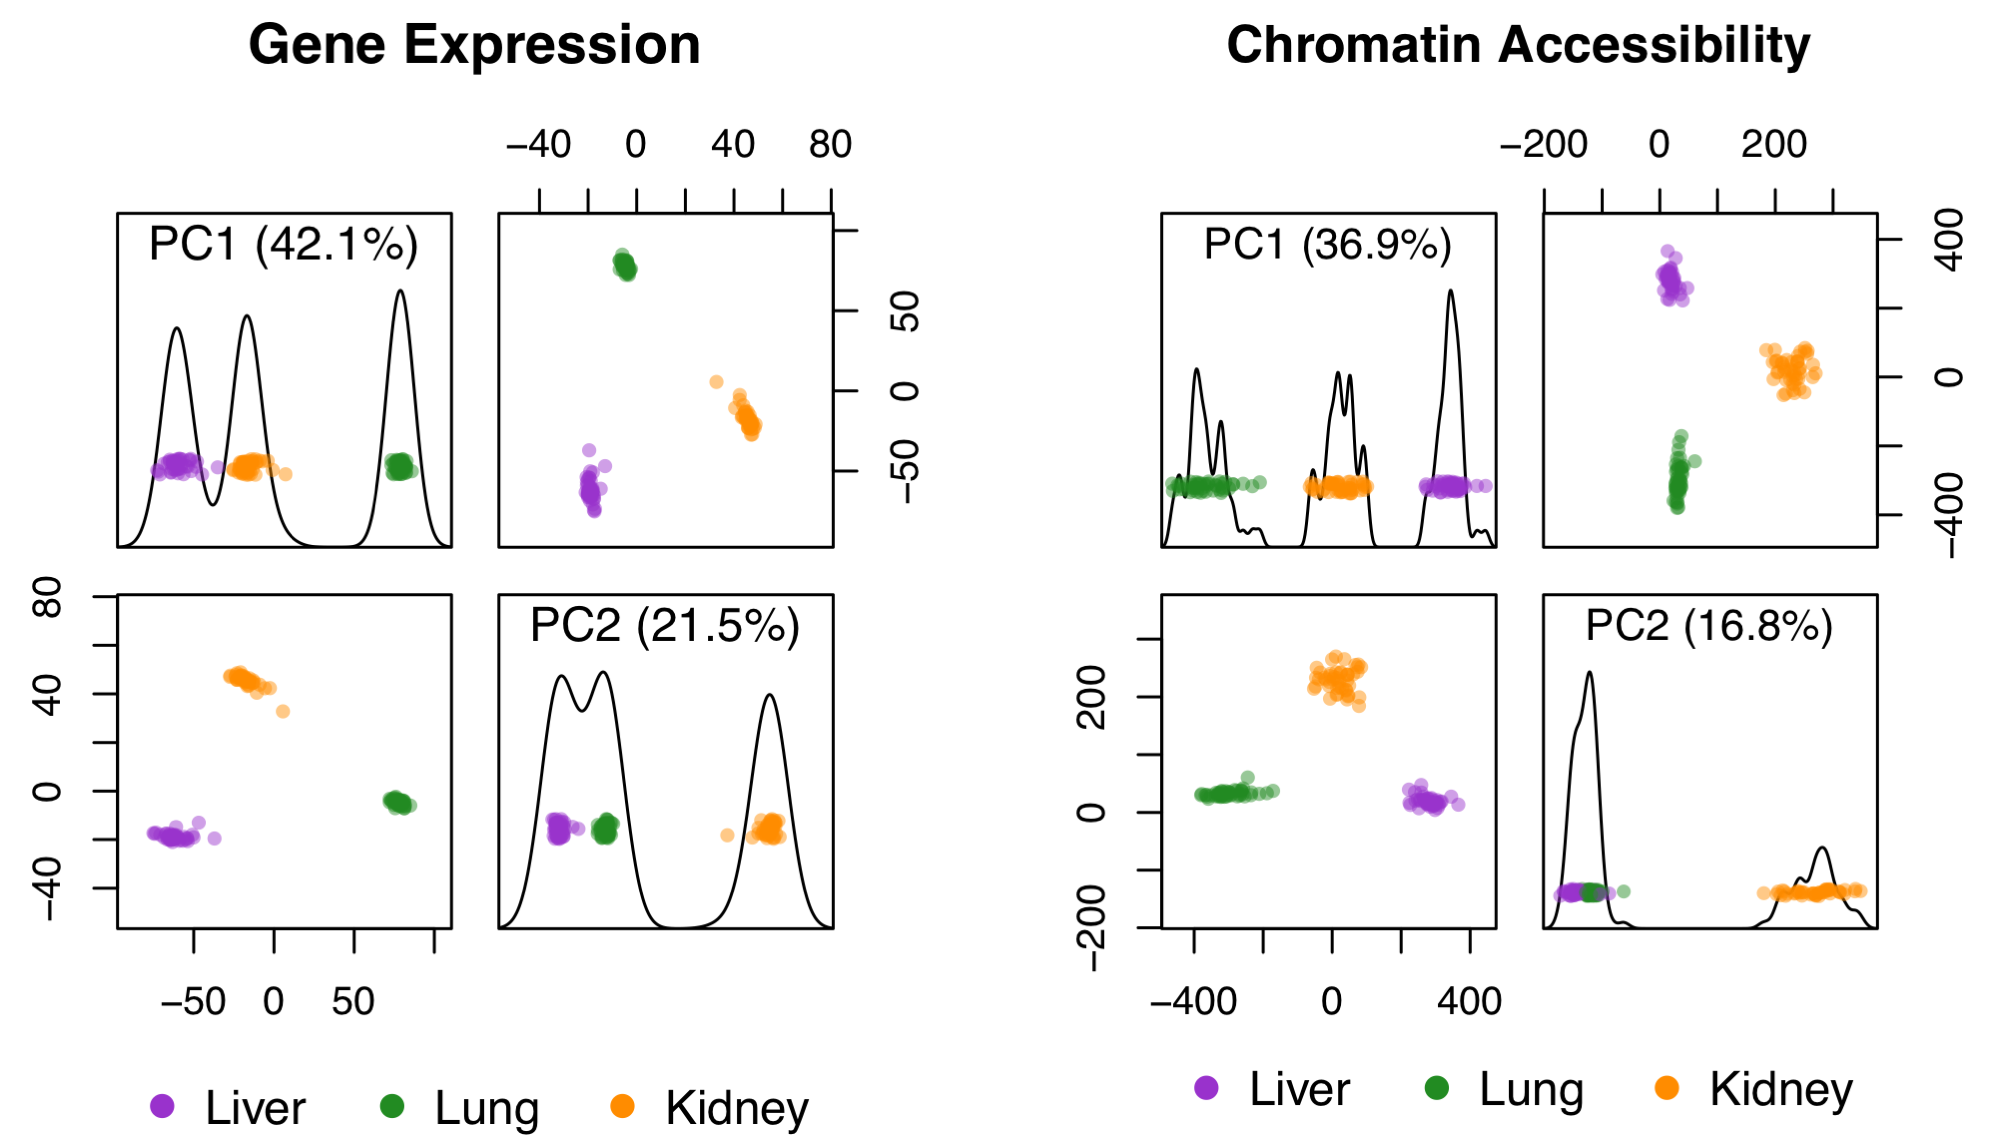
\includegraphics[width=0.8\textwidth, trim={0in 0in 0in 0in}, clip]{figs/pca_plot.png}
\caption{\textbf{Principle components analysis identifies tissue type as key source of variation for gene expression and chromatin accessibility.} 
Molecular traits for liver (pink), lung (green), and kidney (orange) tissue samples were derived from RNA-seq and ATAC-seq data. Principal components (PC) 1 and 2 capture a majority of the variation and show a greater amount of between tissue variability than within tissue variability. \label{fig:pca_plots}}
\end{figure*}

\clearpage

\begin{figure*}[hp]
\renewcommand{\familydefault}{\sfdefault}\normalfont
\centering
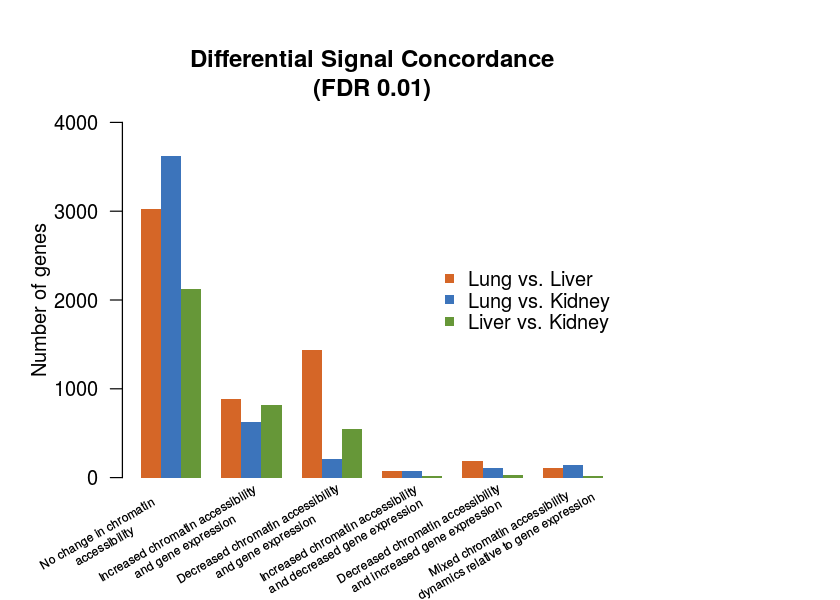
\includegraphics[width=0.8\textwidth, trim={0in 0in 0in 0in}, clip]{figs/diff_concordance.png}
\caption{\textbf{Concordance between differentially expressed genes and differentially accessible regions in between-tissue comparisons.} 
Genes were categorized by the direction of the difference in expression and chromatin accessibility in their promoter regions.\label{fig:diff_concordance}}
\end{figure*}

\clearpage

\begin{figure*}[hp]
\renewcommand{\familydefault}{\sfdefault}\normalfont
\centering
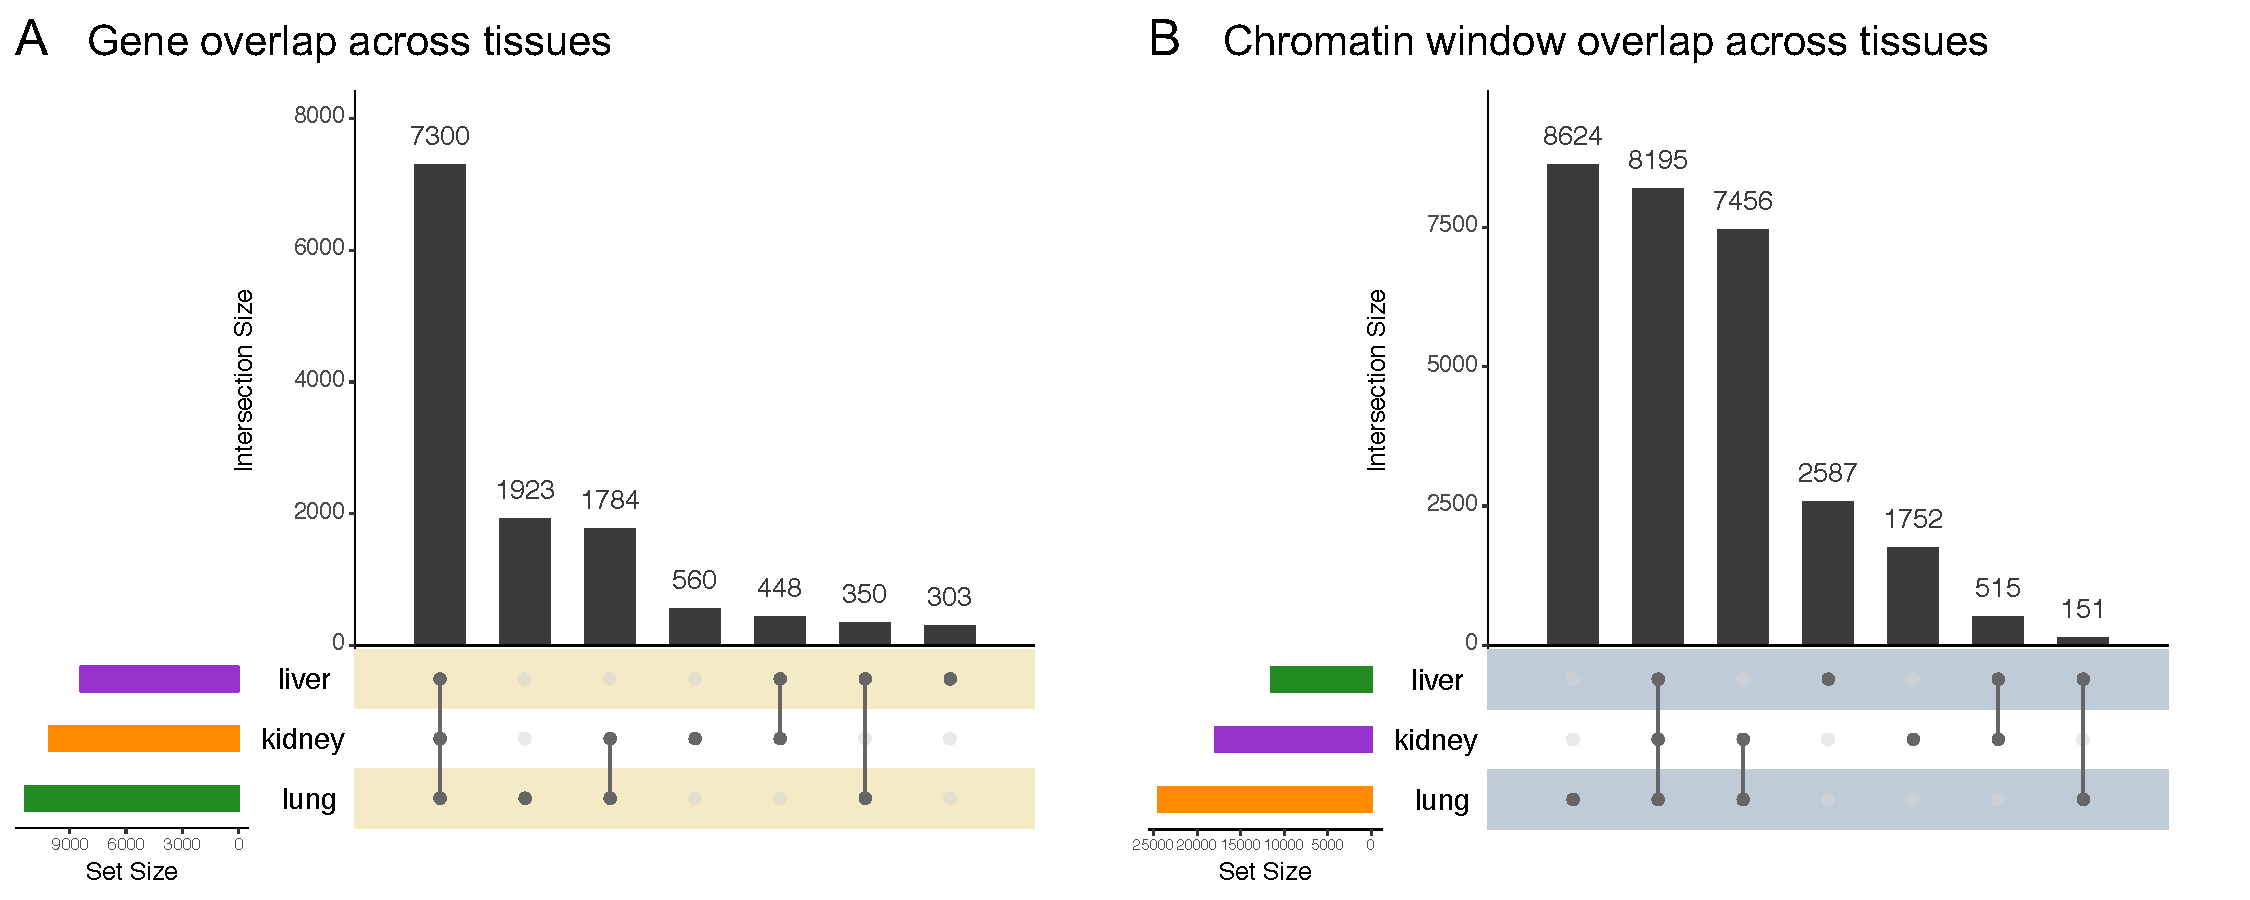
\includegraphics[width=\textwidth, trim={0in 0in 0in 0in}, clip]{figs/upset_genes_chromatin.pdf}
\caption{\textbf{Overlap across tissues of genes (A) and chromatin windows (B) used for QTL analysis.} 
Sequence traits were filtered to remove outcomes more likely to cause in spurious QTL signal. Genes with TPM $\le 1$ and chromatin windows with TMP $\le 5$ for $\ge$ 50\% of samples were removed from analysis. After this filtering process, lung had the greatest number of traits analyzed, for both genes and chromatin windows, followed by kidney and then liver. 
\label{fig:upset_genes_chromatin}}
\end{figure*}

\clearpage

\begin{figure*}[hp]
\renewcommand{\familydefault}{\sfdefault}\normalfont
\centering
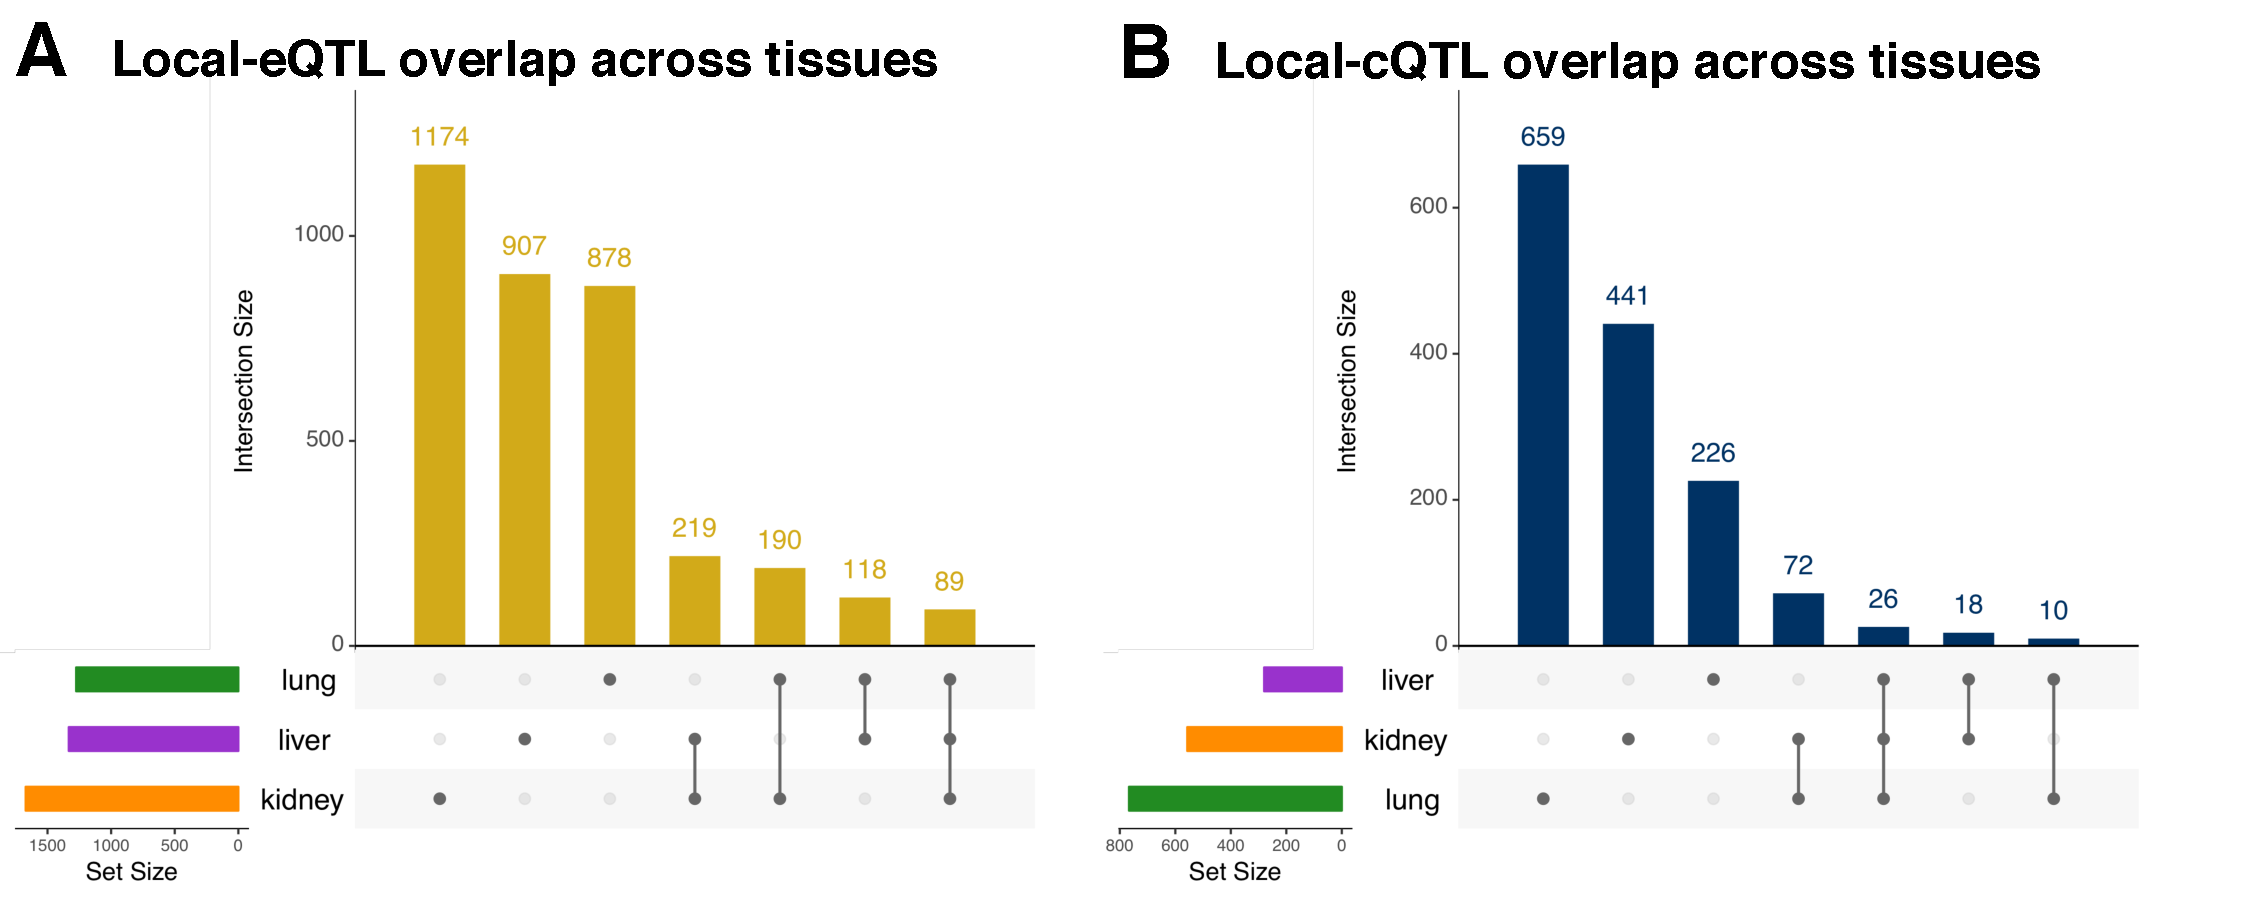
\includegraphics[width=\textwidth, trim={0in 0in 0in 0in}, clip]{figs/upset_eqtl_cqtl.pdf}
\caption{\textbf{Overlap across tissues of genes (A) and chromatin windows (B) with local-QTL detected.} 
The majority of sequence traits with a local-QTL detected were identified in only a single tissue. Kidney had the highest number of local-eQTL, whereas lung had the highest number of local-cQTL. Liver had a relative lack of local-cQTL, which may relate to its having the fewest chromatin windows analyzed (Figure \ref{fig:upset_genes_chromatin}B). Results included local-QTL detected with Analysis G (FDR $<$ 0.1), Analysis C (FDR $<$ 0.1), and Analysis L (genome-wide and chromosome-wide). 
\label{fig:upset_eqtl_cqtl}}
\end{figure*}

\clearpage

\begin{figure*}[hp]
\renewcommand{\familydefault}{\sfdefault}\normalfont
\centering
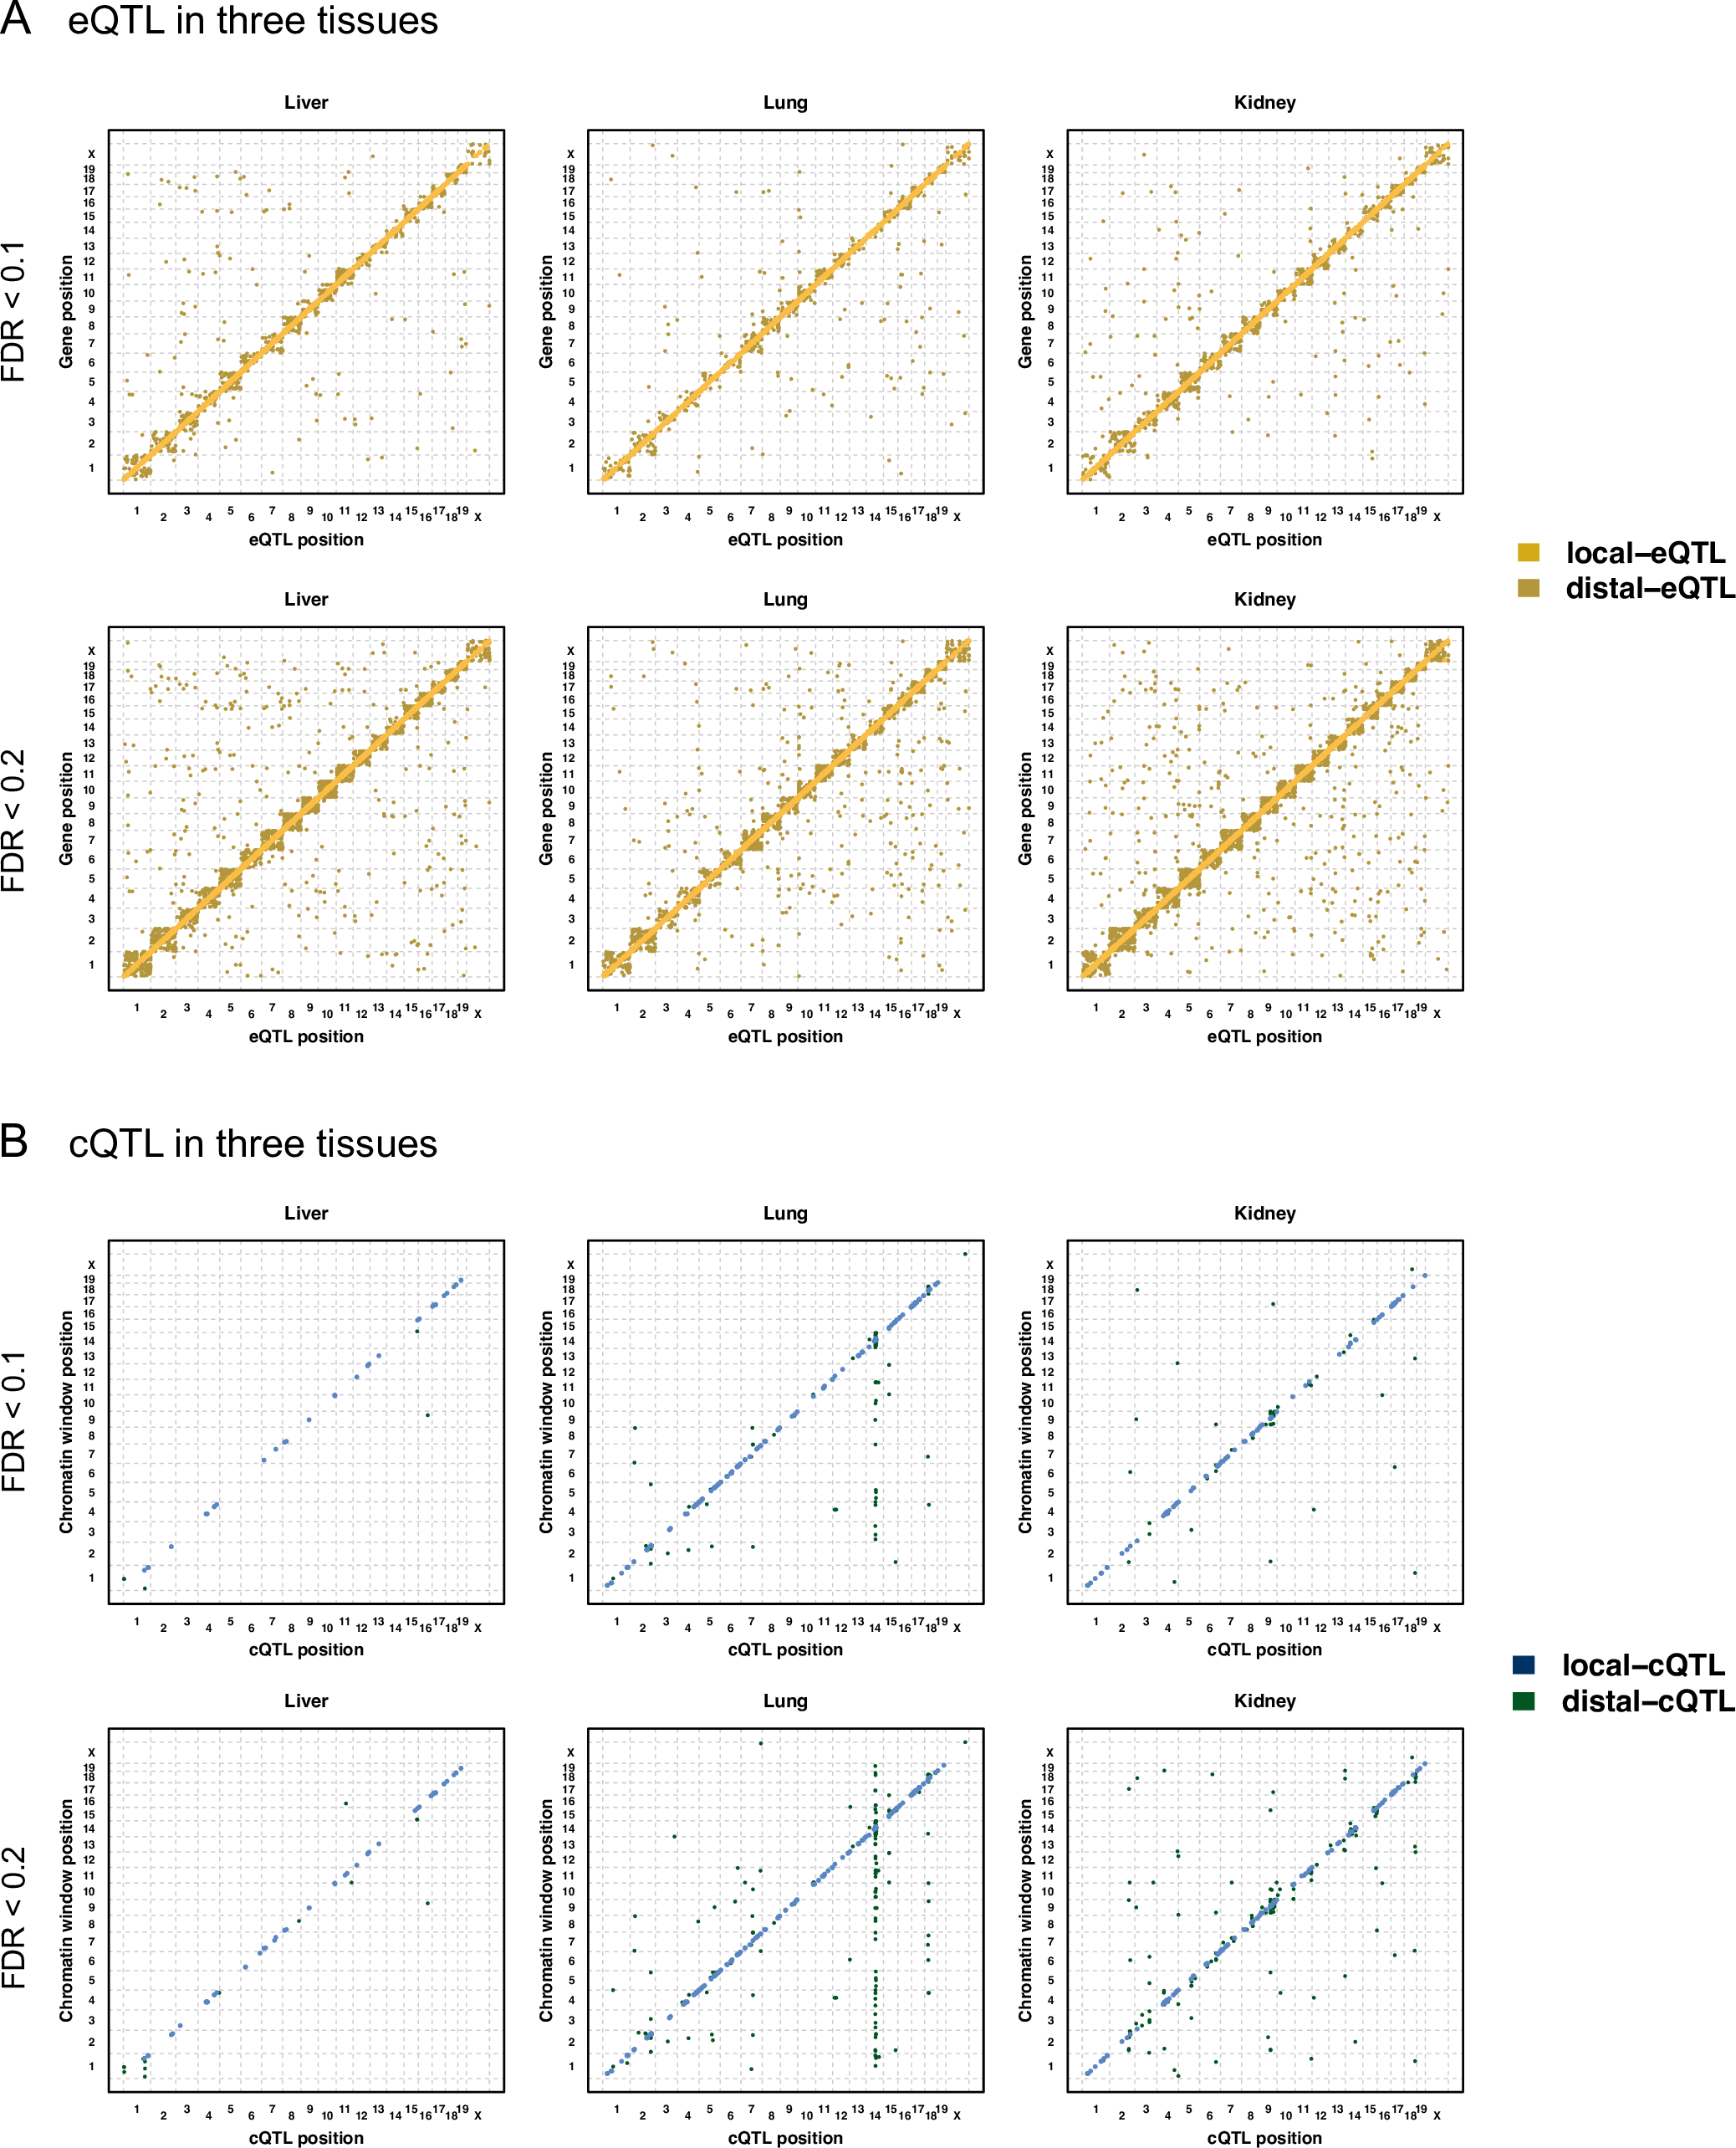
\includegraphics[width=0.8\textwidth, trim={0in 0in 0in 0in}, clip]{figs/qtl_map_supplemental.png}
\caption{\textbf{QTL mapping results using only Analysis G or Analysis C.} 
QTL map plots of eQTL (A) and cQTL (B) with FDR controlled at 0.1 and 0.2 for liver, lung, and kidney. Detected QTL from Analysis G (multi-stage FDR) and Analysis C (chromosome-wide FDR) are included. Analysis C, which uses FDR control for chromosome-wide significant QTL, produces a large number of intra-chromosomal distal QTL. The y-axis represents the genomic position of the gene or chromatin site, and the x-axis represents the genomic position of the QTL. Local-QTL appear as dots along the diagonal.
\label{fig:grid_fdr_plot}}
\end{figure*}

\clearpage

\begin{figure*}[hp]
\renewcommand{\familydefault}{\sfdefault}\normalfont
\centering
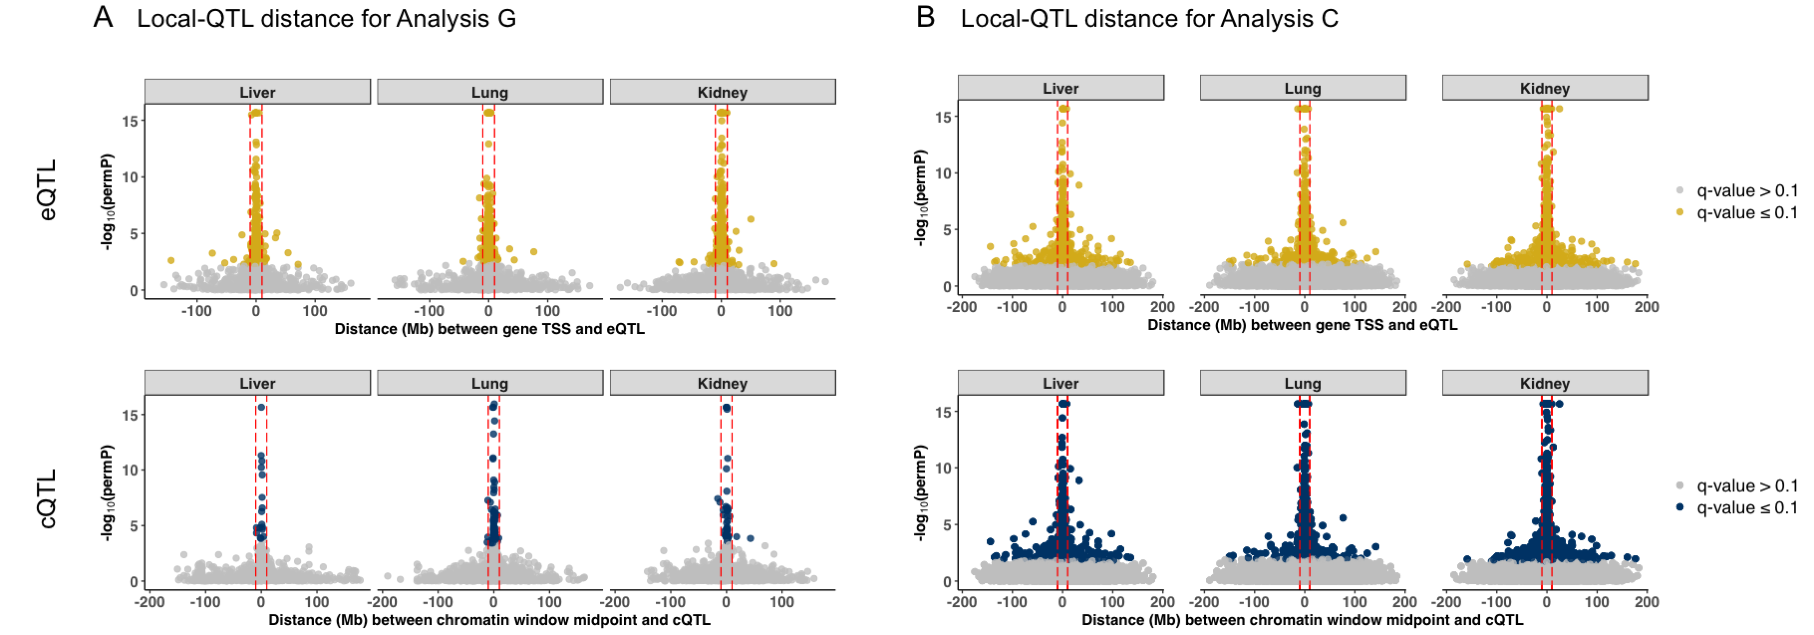
\includegraphics[width=\textwidth]{figs/qtl_distance_all.png}
\caption{\textbf{Highly significant QTL map nearby the gene TSS and chromatin window midpoint.} 
The permutation-based $p$-value (permP) from Analyses G (A) and C (B) for eQTL and cQTL by the distance (Mb) from the gene TSS and the midpoint of the chromatin site. Inter-chromosomal distal-QTL are not included. The red dashed lines represent 10Mb upstream and downstream of the gene TSS or the midpoint of the chromatin site for classifying QTL as local or distal. Significant signals (yellow or blue), based on $q\text{-value} \le 0.1$, are largely local. Analysis C detects many more intra-chromosomal distal-QTL.
\label{fig:dist_all}}
\end{figure*}

\clearpage

\begin{figure*}[hp]
\renewcommand{\familydefault}{\sfdefault}\normalfont
\centering
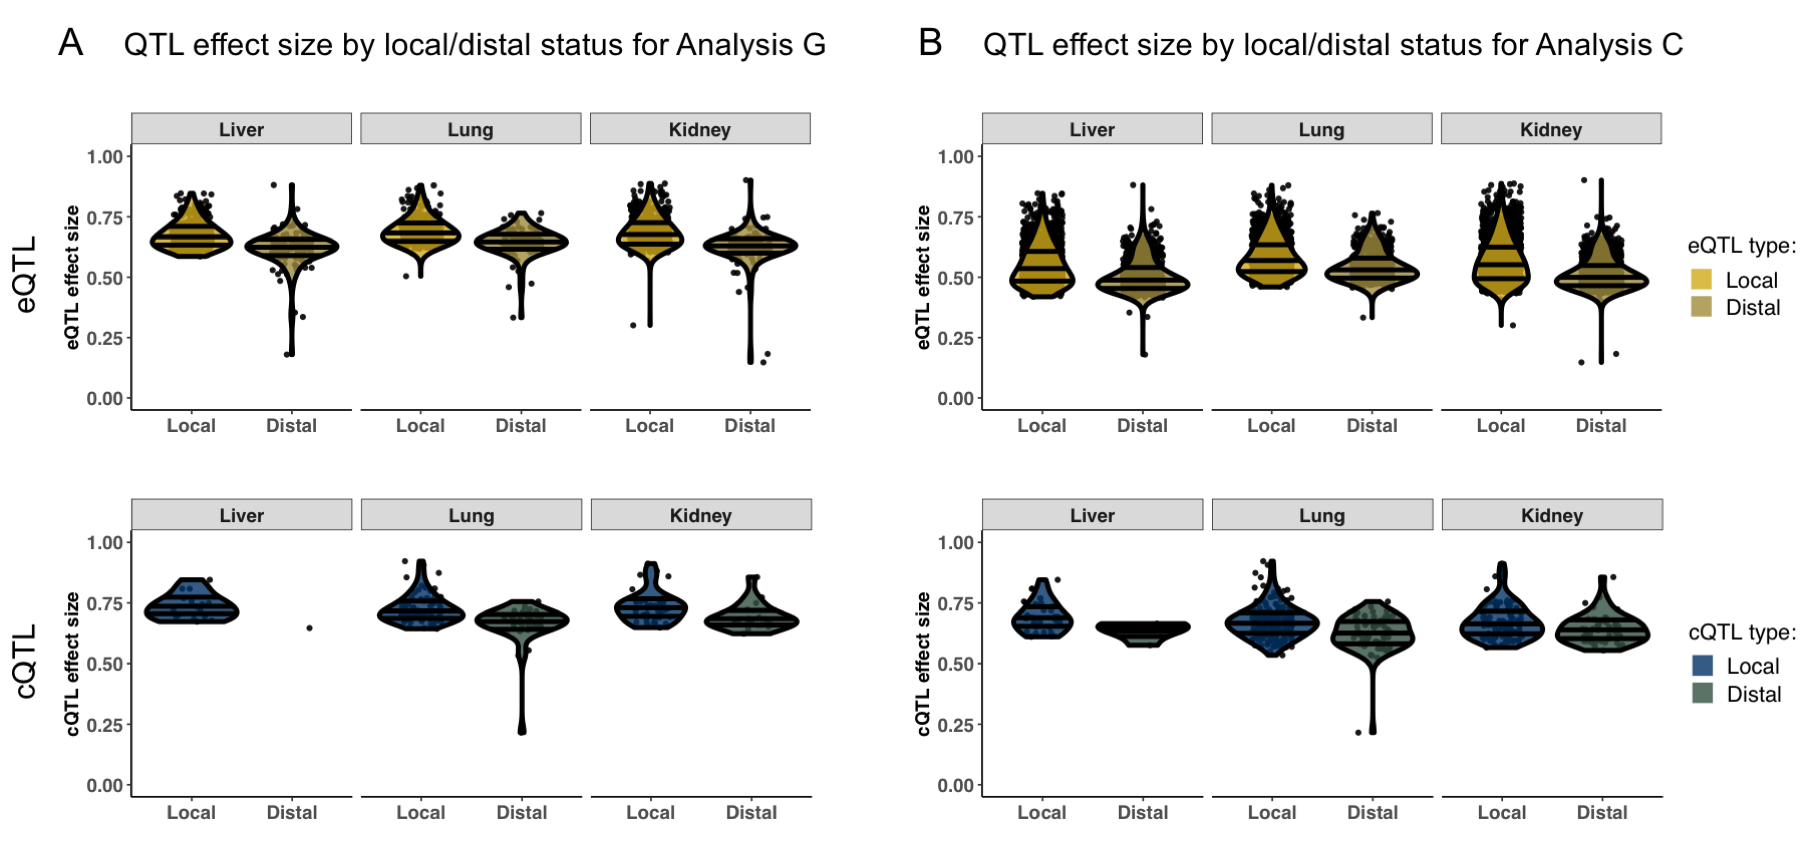
\includegraphics[width=0.9\textwidth, trim={0in 0.25in 0in 0in}, clip]{figs/qtl_effect_sizes_local_v_distal.png}
\caption{\textbf{QTL effect sizes by local/distal status.} 
Each dot represents a QTL detected through either Analyses G (A) or C (B) with FDR < 0.1. The three horizontal bars represent the 25\textsuperscript{th}, 50\textsuperscript{th}, and 75\textsuperscript{th} quantiles of QTL effect sizes for all local-QTL per tissue. More local-eQTL are detected and have higher effects than distal-QTL. Analysis C detects a large number of intra-chromosomal distal-QTL that Analysis G does not, many of which have low effect sizes. Effect size estimates are based on a fixed effects model.
\label{fig:qtl_effect_sizes_local_v_distal}}
\end{figure*}

\begin{figure*}[hp]
\renewcommand{\familydefault}{\sfdefault}\normalfont
\centering
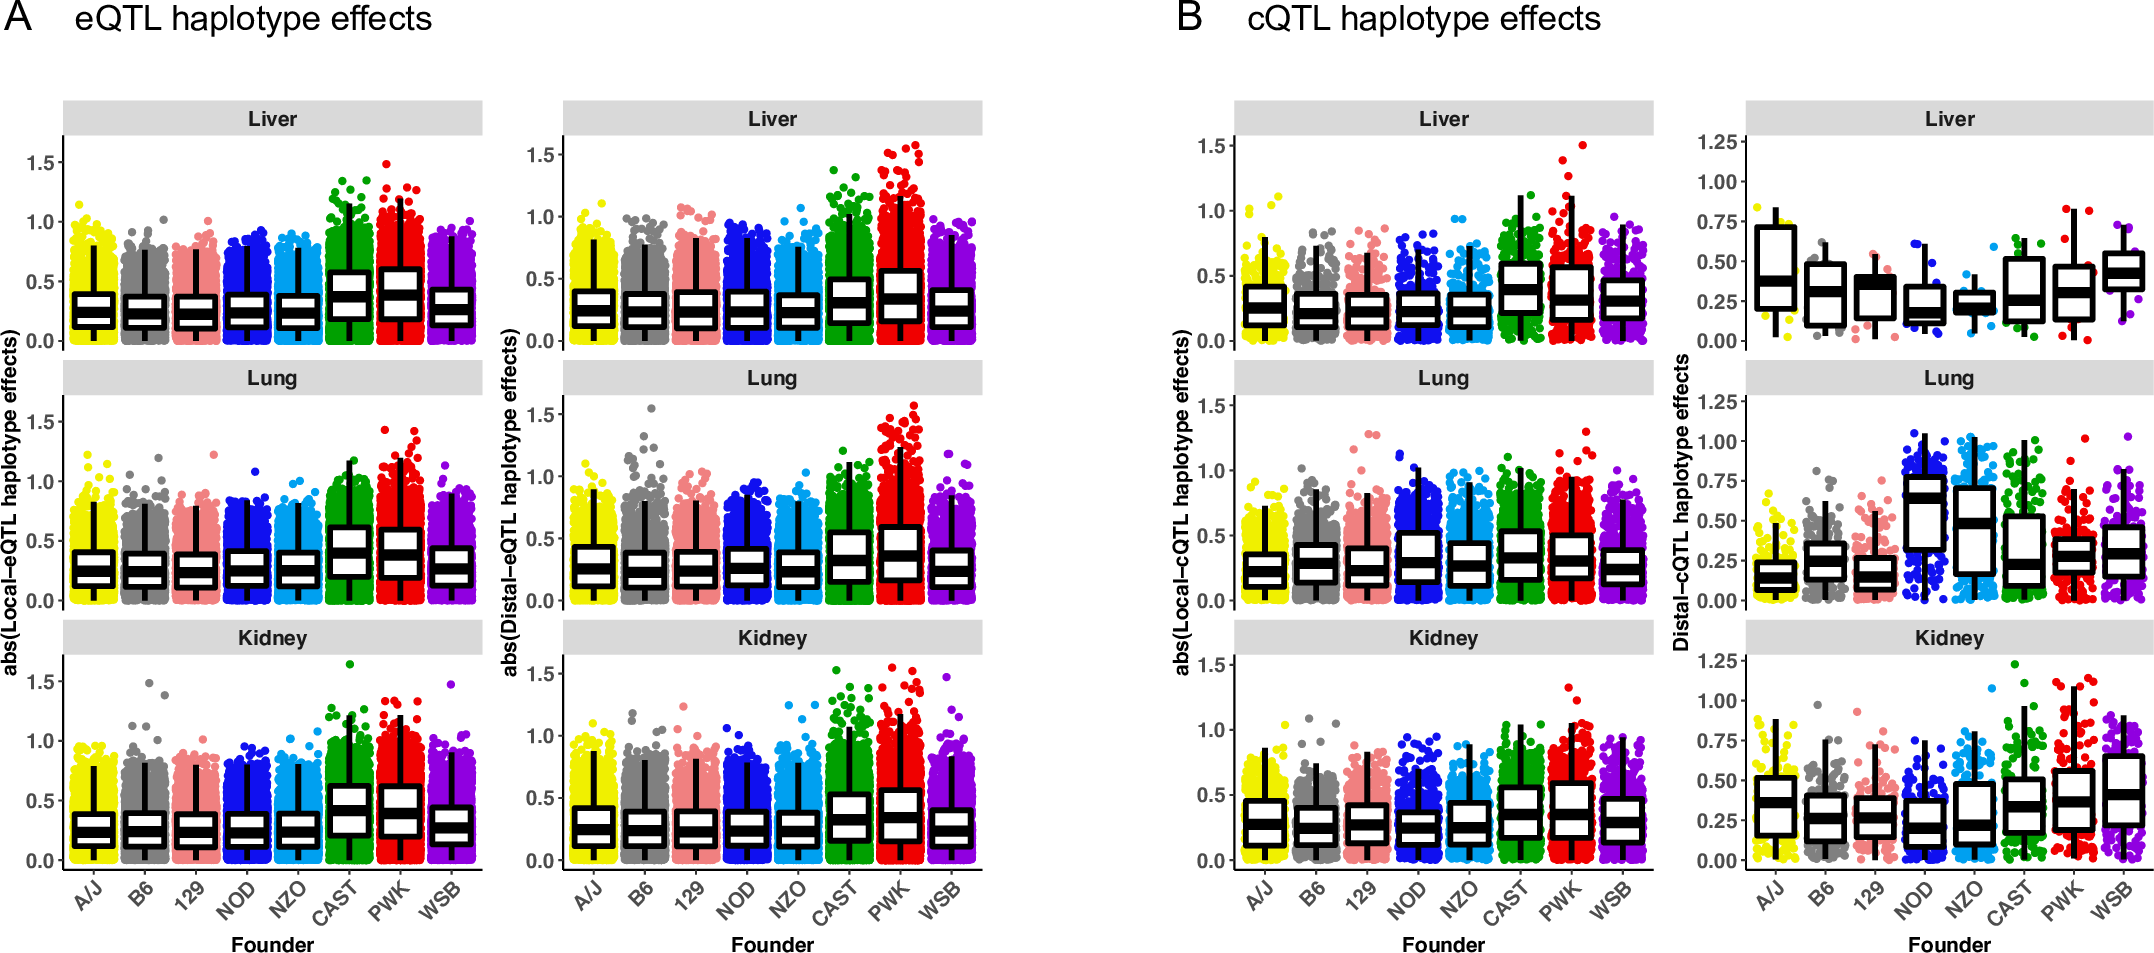
\includegraphics[width=\textwidth, trim={0in 0in 0in 0in}, clip]{figs/all_qtl_effects_abs.png}
\caption{\textbf{CAST and PWK haploytpes have more extreme haplotype effects for eQTL and cQTL compared with the other strains.} 
Haplotype effects were estimated as BLUPs, which are constrained and centered around 0. Each QTL is represented by an 8-element effect vector. Founders with more extreme effects are identified by comparing the absolute values of effects. Haploytpe effects for eQTL (A() are are similar to cQTL (B). Trends are unstable in distal-cQTL because so few are identified.
\label{fig:qtl_effects_abs}}
\end{figure*}

\clearpage

\begin{figure*}[hp]
\renewcommand{\familydefault}{\sfdefault}\normalfont
\centering
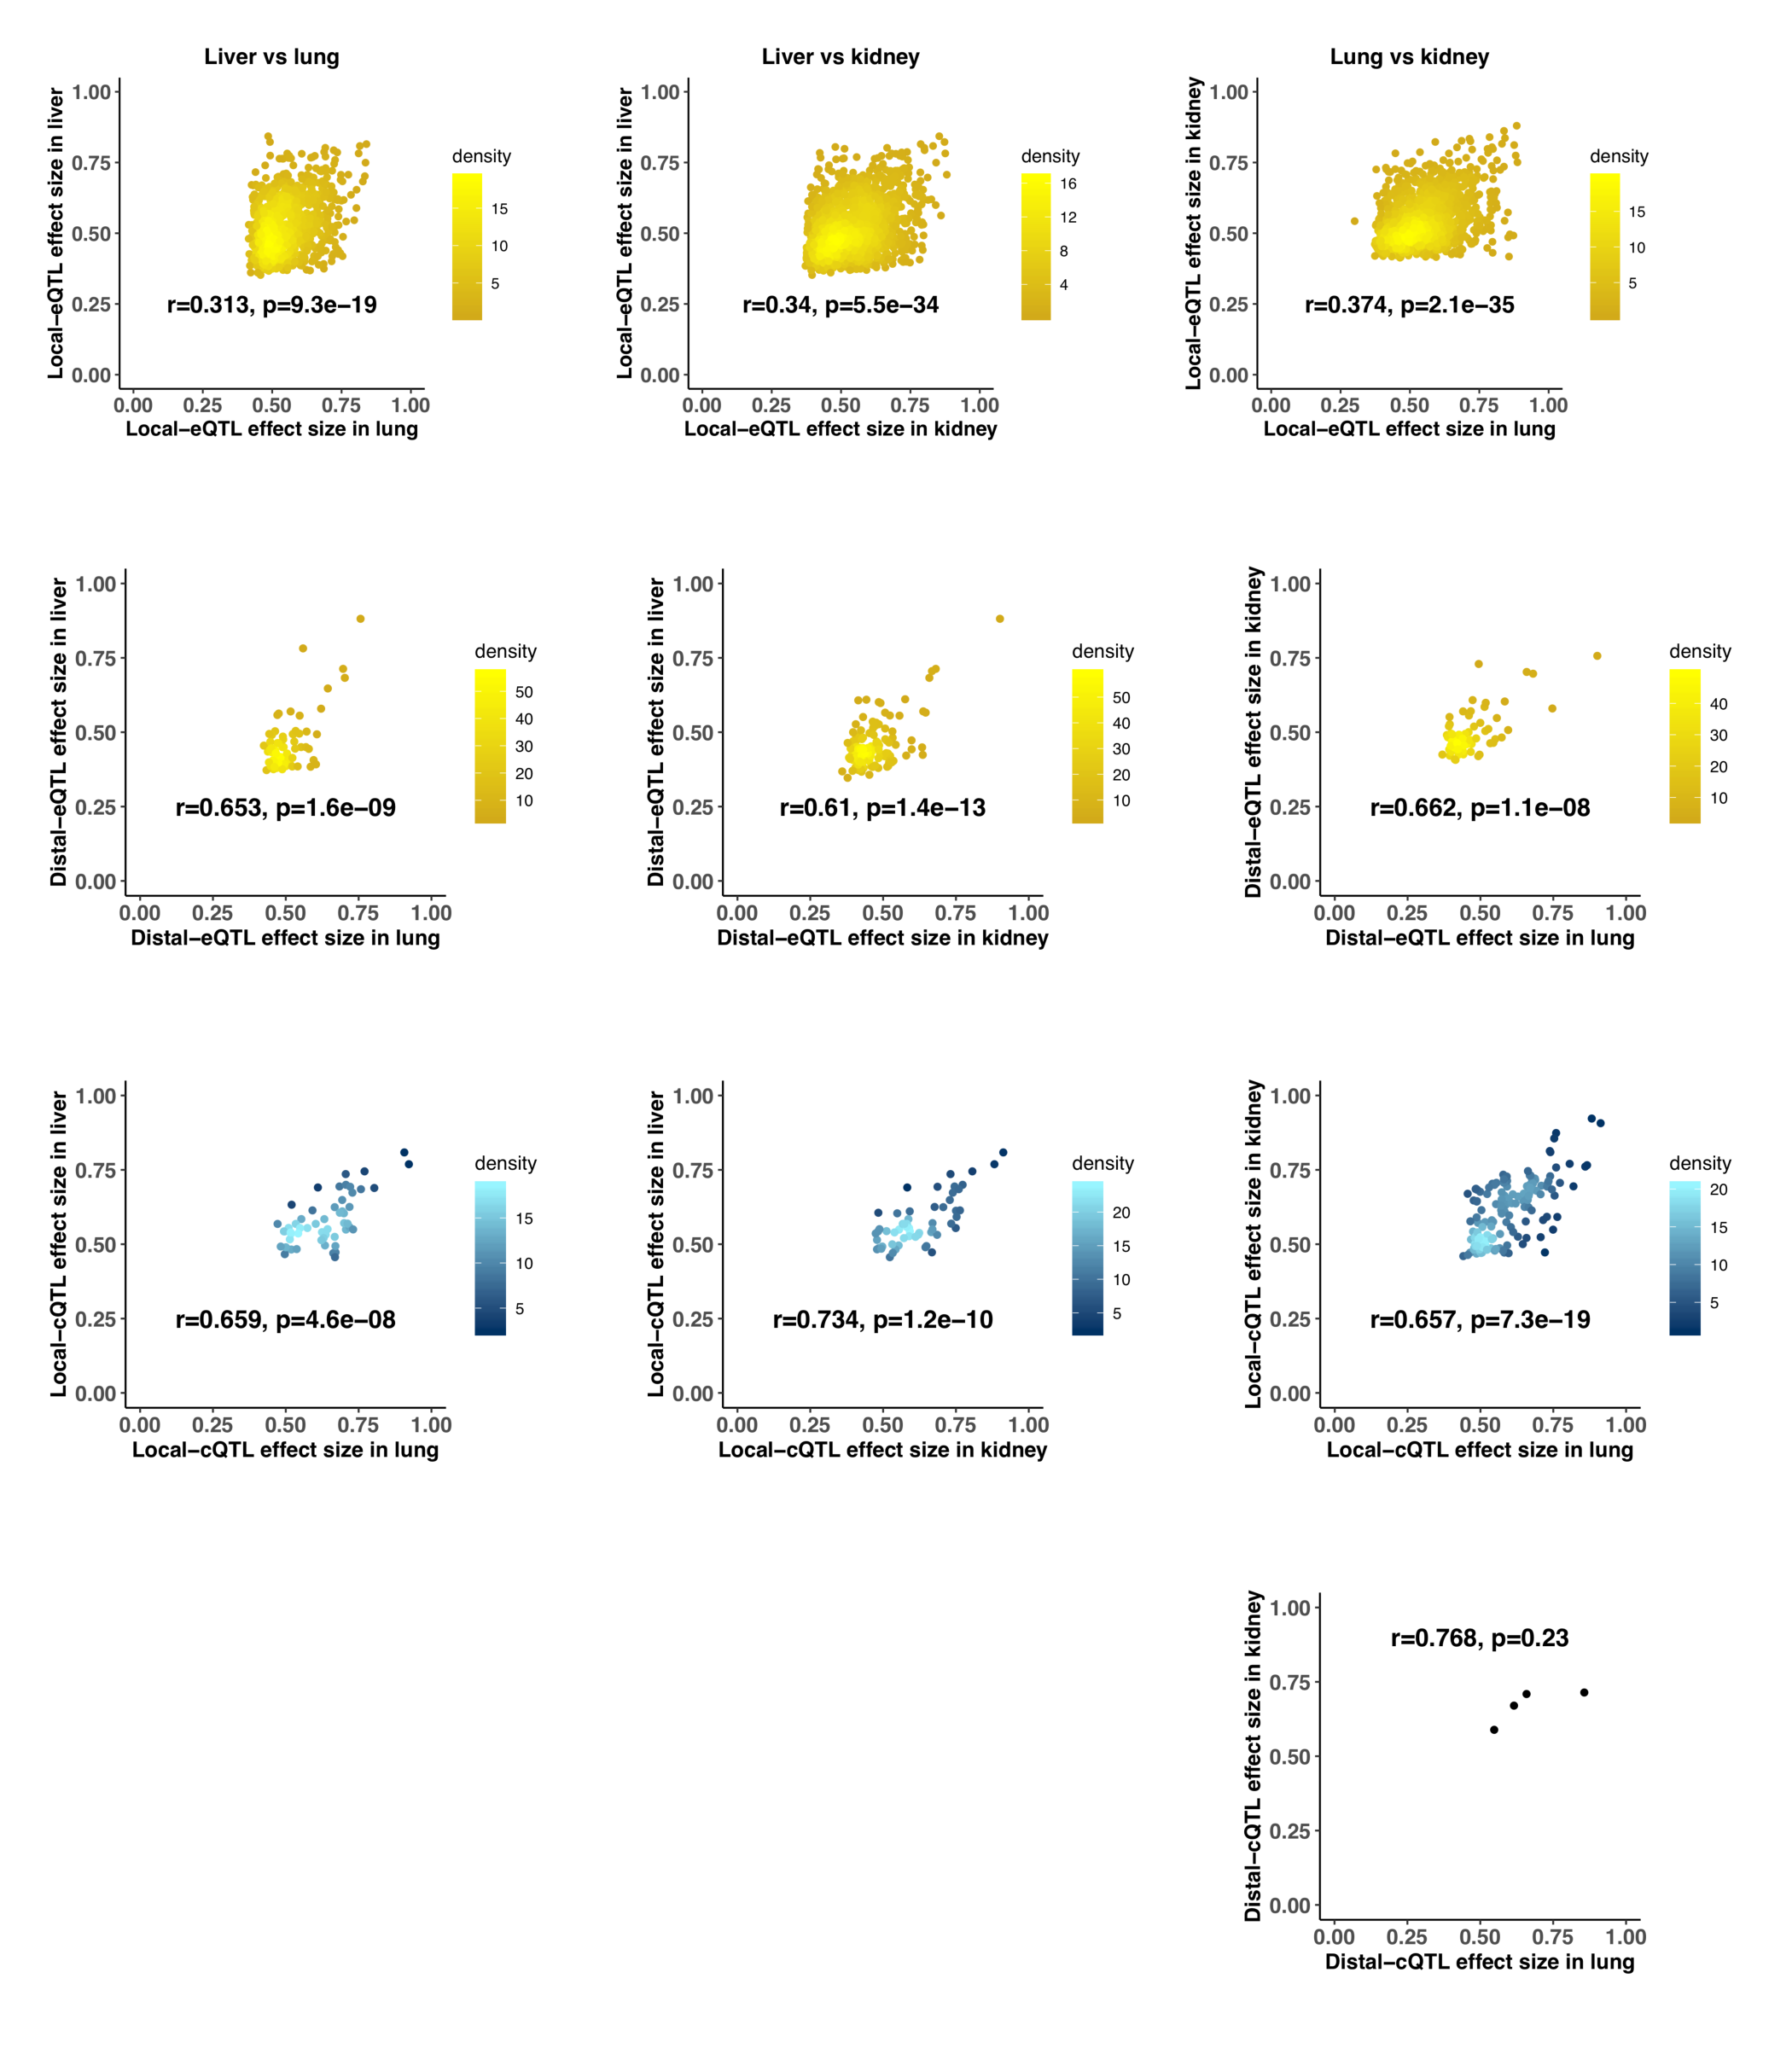
\includegraphics[width=0.9\textwidth, trim={0in 0in 0in 0in}, clip]{figs/effect_size_by_effect_size.pdf}
\caption{\textbf{Effect sizes between cross-tissue QTL pairs are lowly but significantly correlated.} 
Comparisons of QTL effects sizes between (liver/lung) are in the left column, (liver/kidney) middle column, and (lung/kidney) right column. eQTL are yellow and cQTL are blue. Local-eQTL are plotted in the top row, distal-eQTL in the second row, local-cQTL in the third row, and distal-cQTL in the bottom row, with only four pairs detected in (lung/kidney). 
\label{fig:qtl_effect_size_comparison}}
\end{figure*}

\clearpage

\begin{figure*}[hp]
\renewcommand{\familydefault}{\sfdefault}\normalfont
\centering
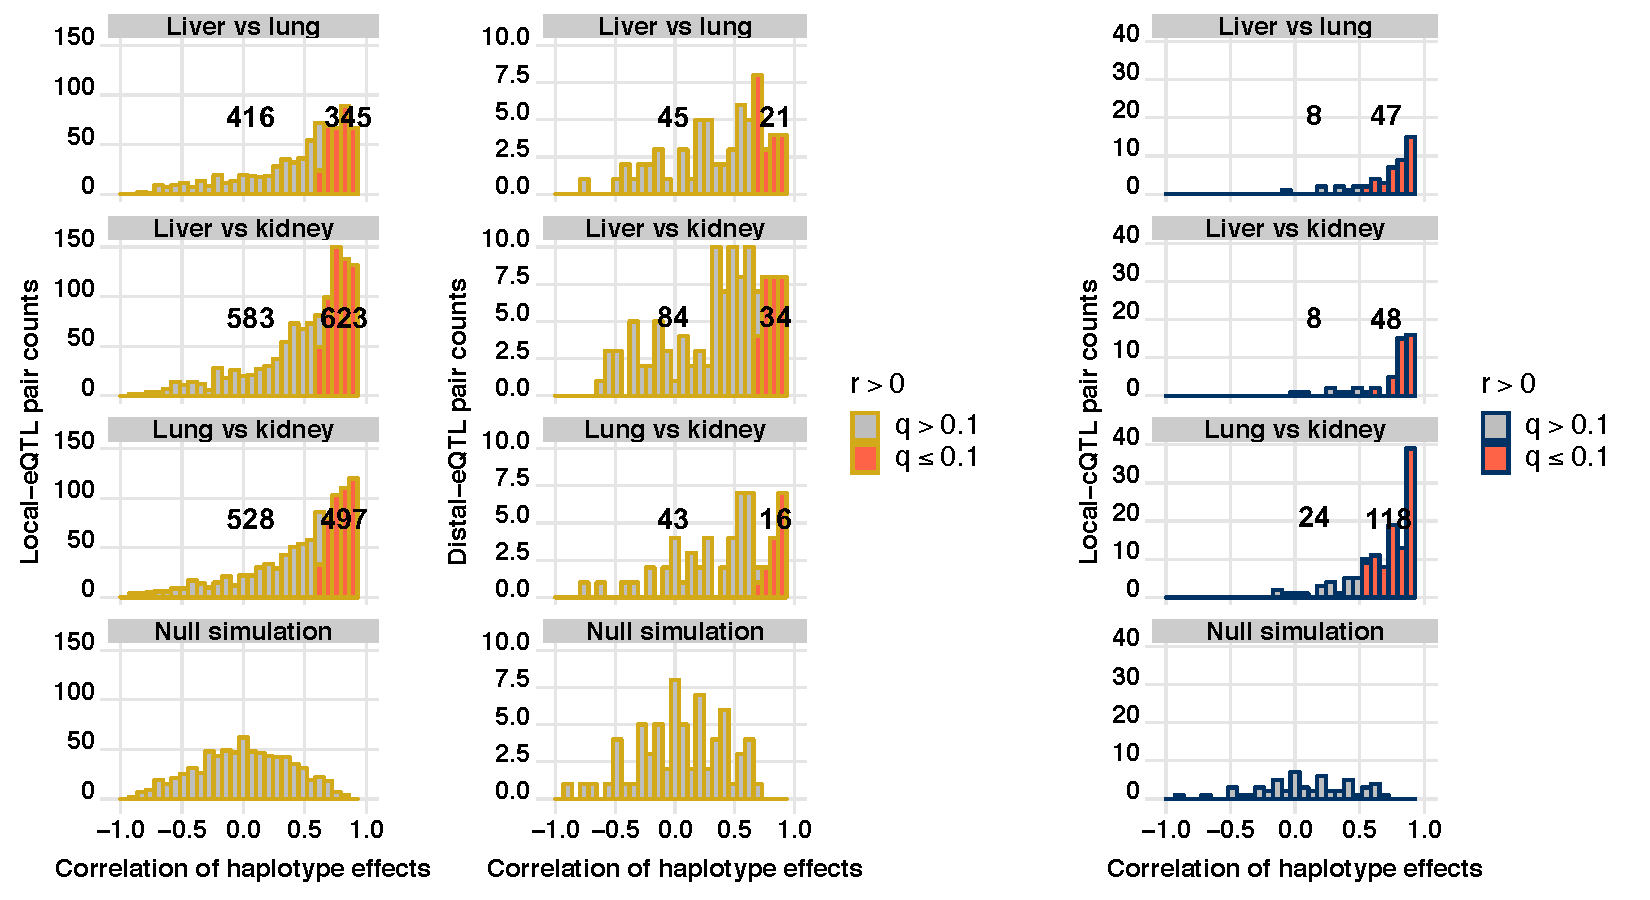
\includegraphics[width=\textwidth, trim={0in 0in 0in 0in}, clip]{figs/qtl_pair_cor_histograms.pdf}
\caption{\textbf{Consistent genetic regulation of gene expression and chromatin accessibility observed across tissues.} 
Enrichment of significantly correlated founder haplotype effects detected in QTL pairs for gene expression and chromatin accessibility. Pairs of QTL observed in multiple tissues were defined for local-eQTL (left column), distal-eQTL (middle column), and local-cQTL (right column). Only four pairs of distal-cQTL were observed, all shared between lung and kidney. A right-tailed test the correlation between founders effects ($H_{A}: r > 0$) was performed for each QTL pair, producing $p$-values that were then FDR adjusted. Null simulations of uncorrelated 8-element vector pairs for each class of QTL and pairwise tissue comparison emphasize the observed enrichment in correlated founder effects between QTL pairs.  
\label{fig:qtl_pair_histograms}}
\end{figure*}

\clearpage

\begin{figure*}[hp]
\renewcommand{\familydefault}{\sfdefault}\normalfont
\centering
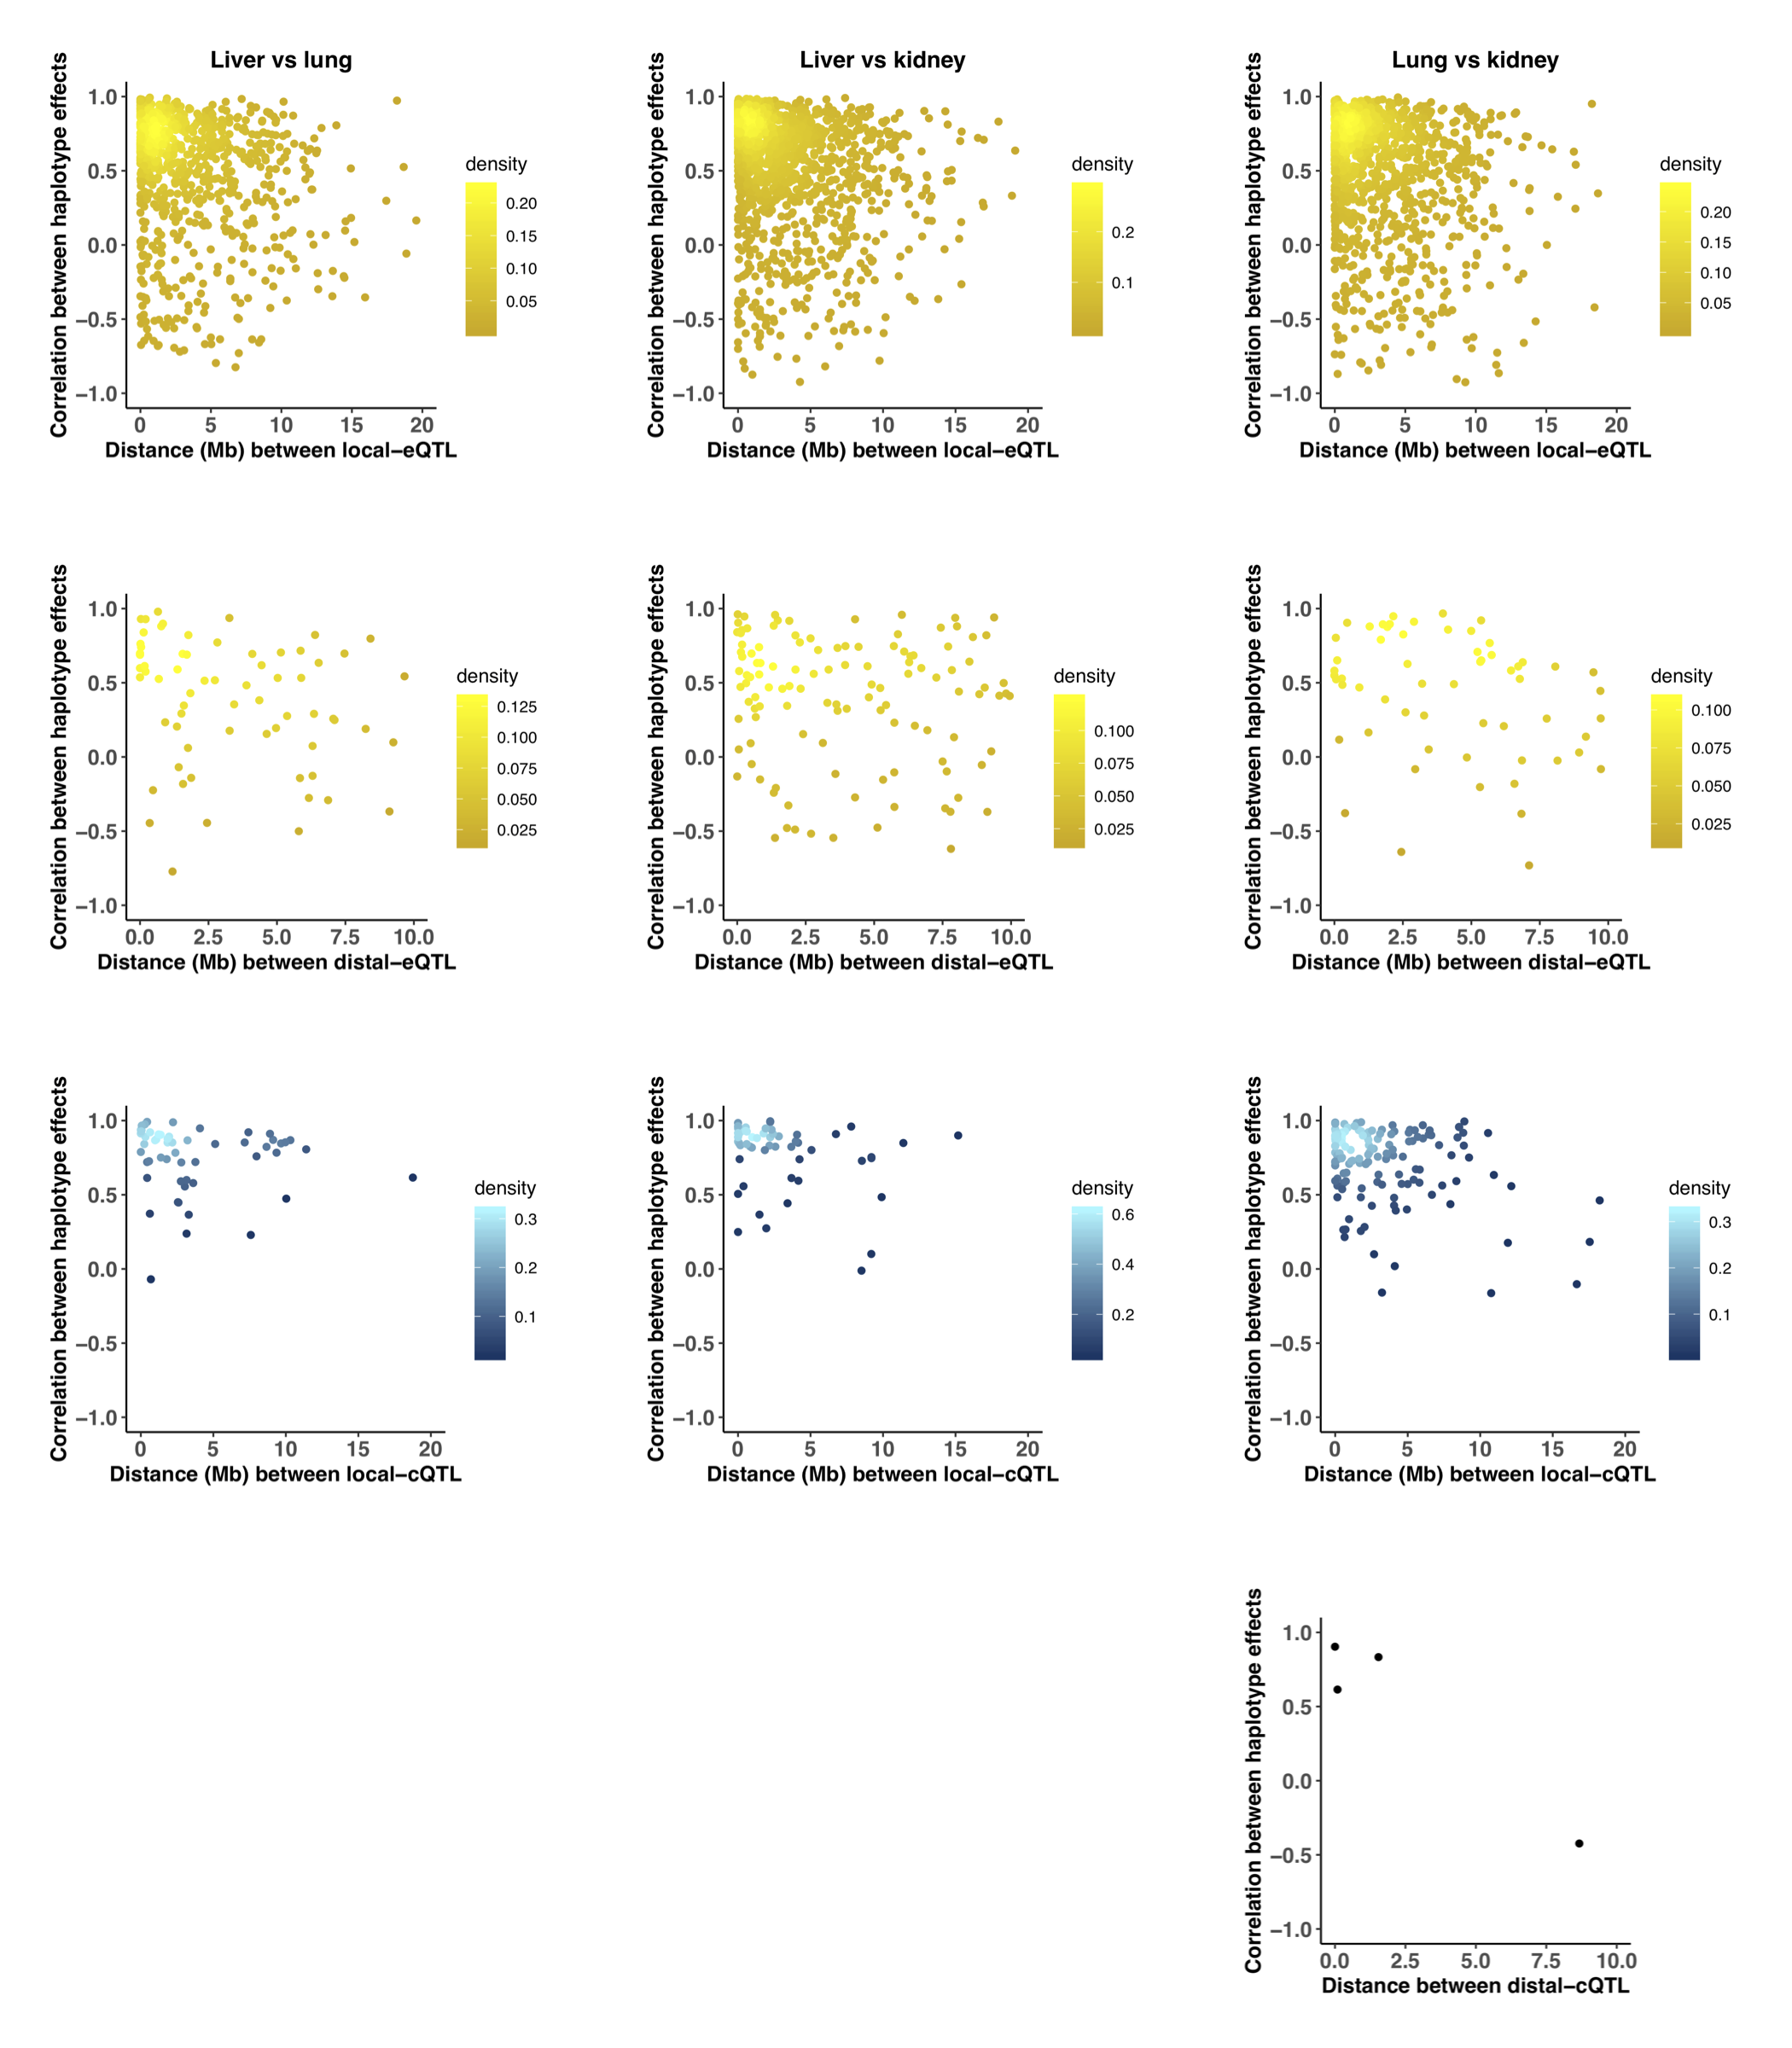
\includegraphics[width=0.9\textwidth, trim={0in 0in 0in 0in}, clip]{figs/effect_size_cor_by_dist.png}
\caption{\textbf{Cross-tissue QTL pairs with highly correlated founder haplotype effects map proximally to each other.} 
Founder effects were estimated as constrain BLUPs. Pairwise correlations of the 8-element effect vectors were calculated for QTL pairs, and plotted again the distance between the QTL coordinates inMb for (liver/lung) in the left column, (liver/kidney) in the middle column, and (lung/kidney) in the right column. Single eQTL and cQTL pairs are represented as a yellow and blue dots, respectively. Local-eQTL are shown in the top row, distal-eQTL in the second row, local-cQTL in the third row, and distal c-QTL in the bottom row, for which only four pairs were detected in (lung/kidney).
\label{fig:qtl_cor_by_distance_comparison}}
\end{figure*}

\clearpage

\begin{figure*}[hp]
\renewcommand{\familydefault}{\sfdefault}\normalfont
\centering
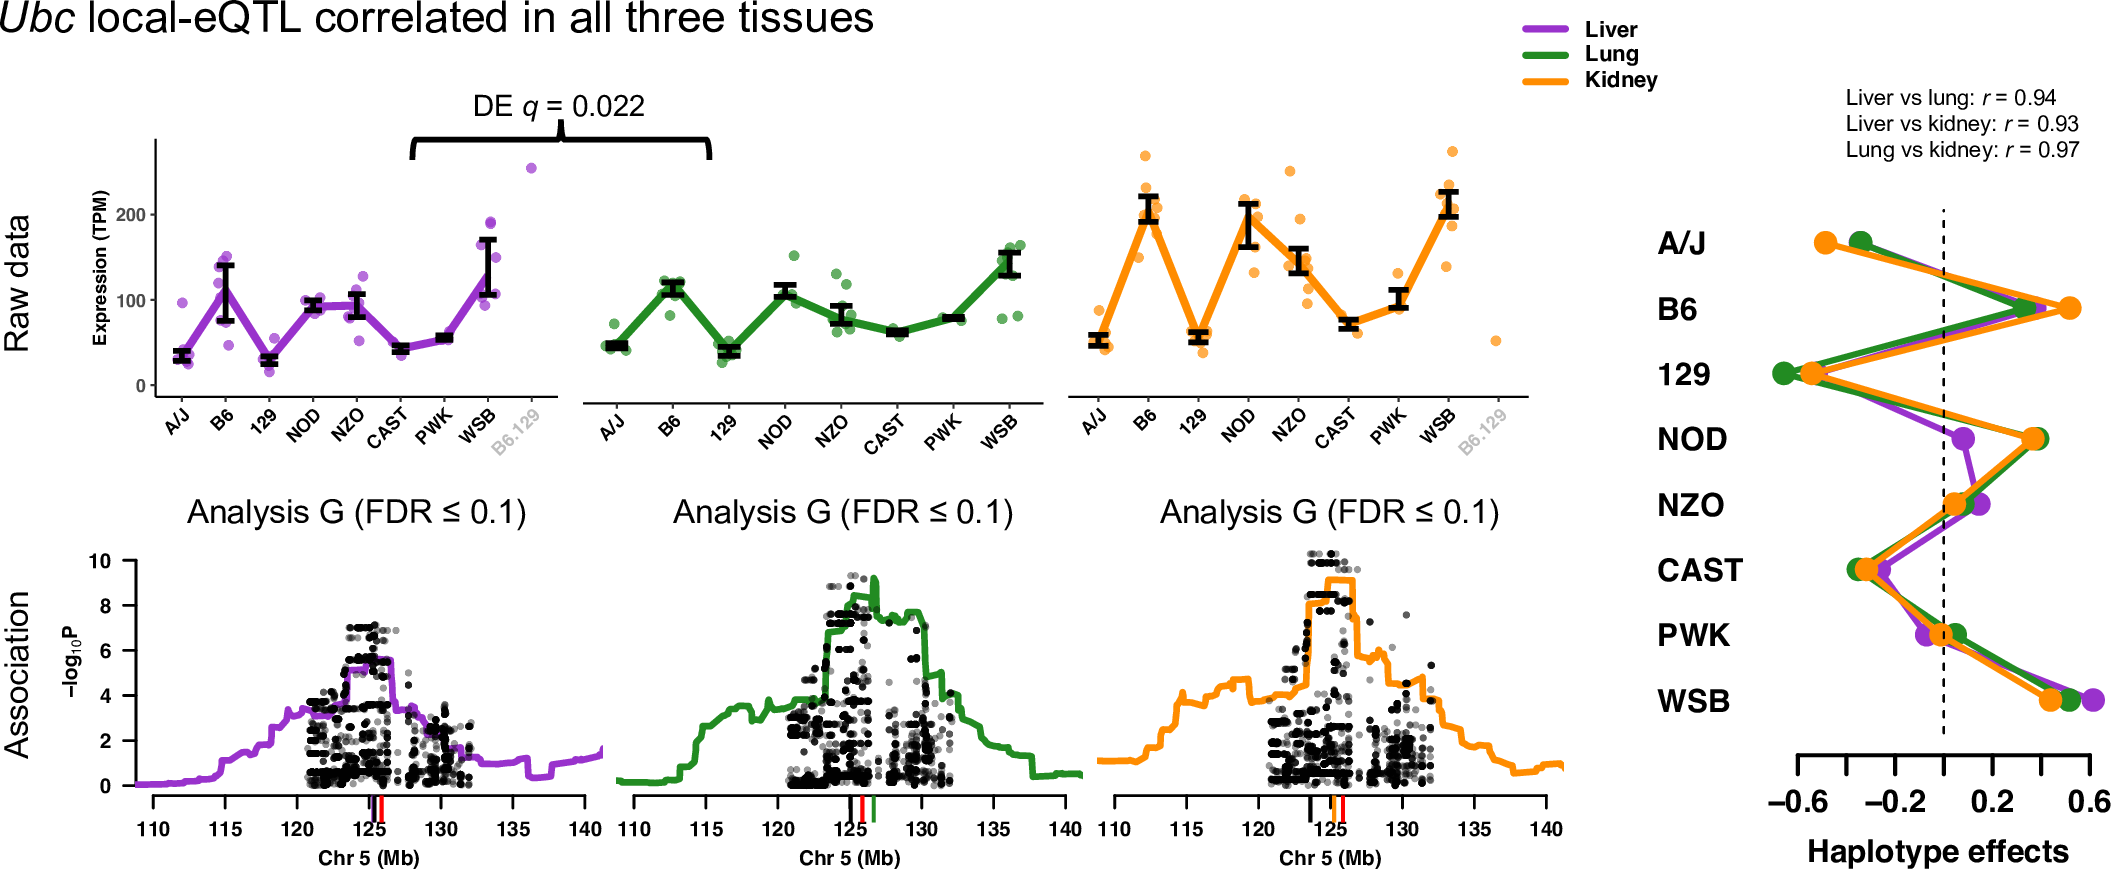
\includegraphics[width=\textwidth, trim={0in 0in 0in 0in}, clip]{figs/ubc_correlated_eqtl.png}
\caption{\textbf{The gene \textit{Ubc} has consistent strong local-eQTL observed in the three tissues.} 
The local-eQTL consistently drove higher expression when the B6, NOD, NZO, and WSB haploytpes were present. Expression levels in liver and lung were found to be significantly different ($q = 0.022$). The estimated haplotype effects, scaled BLUPs, were highly consistent with the expression data, represented as interquartile bars by most likely diplotype. The haplotype and variant associations in the eQTL regions were similar across tissues, suggesting they may represent the same causal origin. The red tick represents the \textit{Ubc} TSS, the black tick represents the peak variant association, and the colored ticks represent the peak haplotype association, each each tissue.
\label{fig:ubc_correlated_eqtl}}
\end{figure*}

\begin{figure*}[hp]
\renewcommand{\familydefault}{\sfdefault}\normalfont
\centering
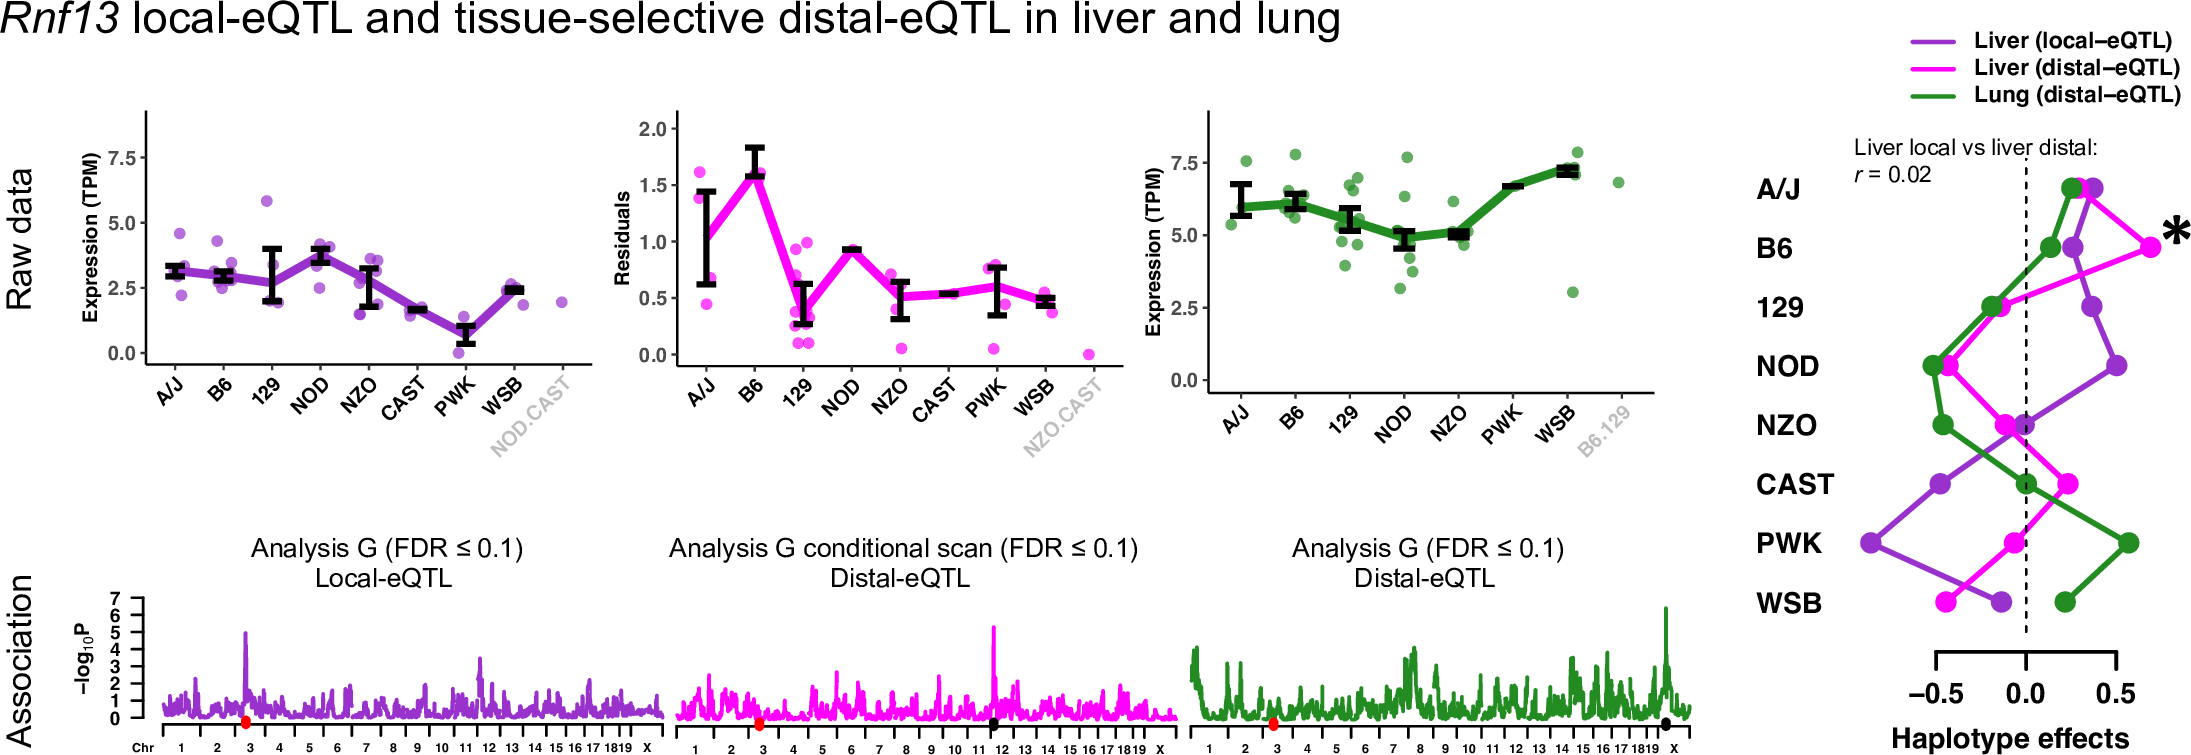
\includegraphics[width=\textwidth, trim={0in 0in 0in 0in}, clip]{figs/rnf13_distal_eqtl.png}
\caption{\textbf{The gene \textit{Rnf13} has tissue-specific patterns of genetic regulation.} 
A strong local-eQTL detected in liver. After conditioning on the local-eQTL, a statistically significant (Analysis G) distal-eQTL was detected on chromosome 12, largely driven by the B6 haplotype, distinct from the local-eQTL. The unique haplotype effect patterns for each eQTL can be seen in both the expression data, represented by interquartile bars by most likely diplotype, and the estimated effects (scaled BLUPs). On the association scans, the red tick marks the \textit{Rnf13} TSS and the black tick marks the location of distal-eQTL.
\label{fig:rnf13_distal_eqtl}}
\end{figure*}

\clearpage

\begin{figure*}[hp]
\renewcommand{\familydefault}{\sfdefault}\normalfont
\centering
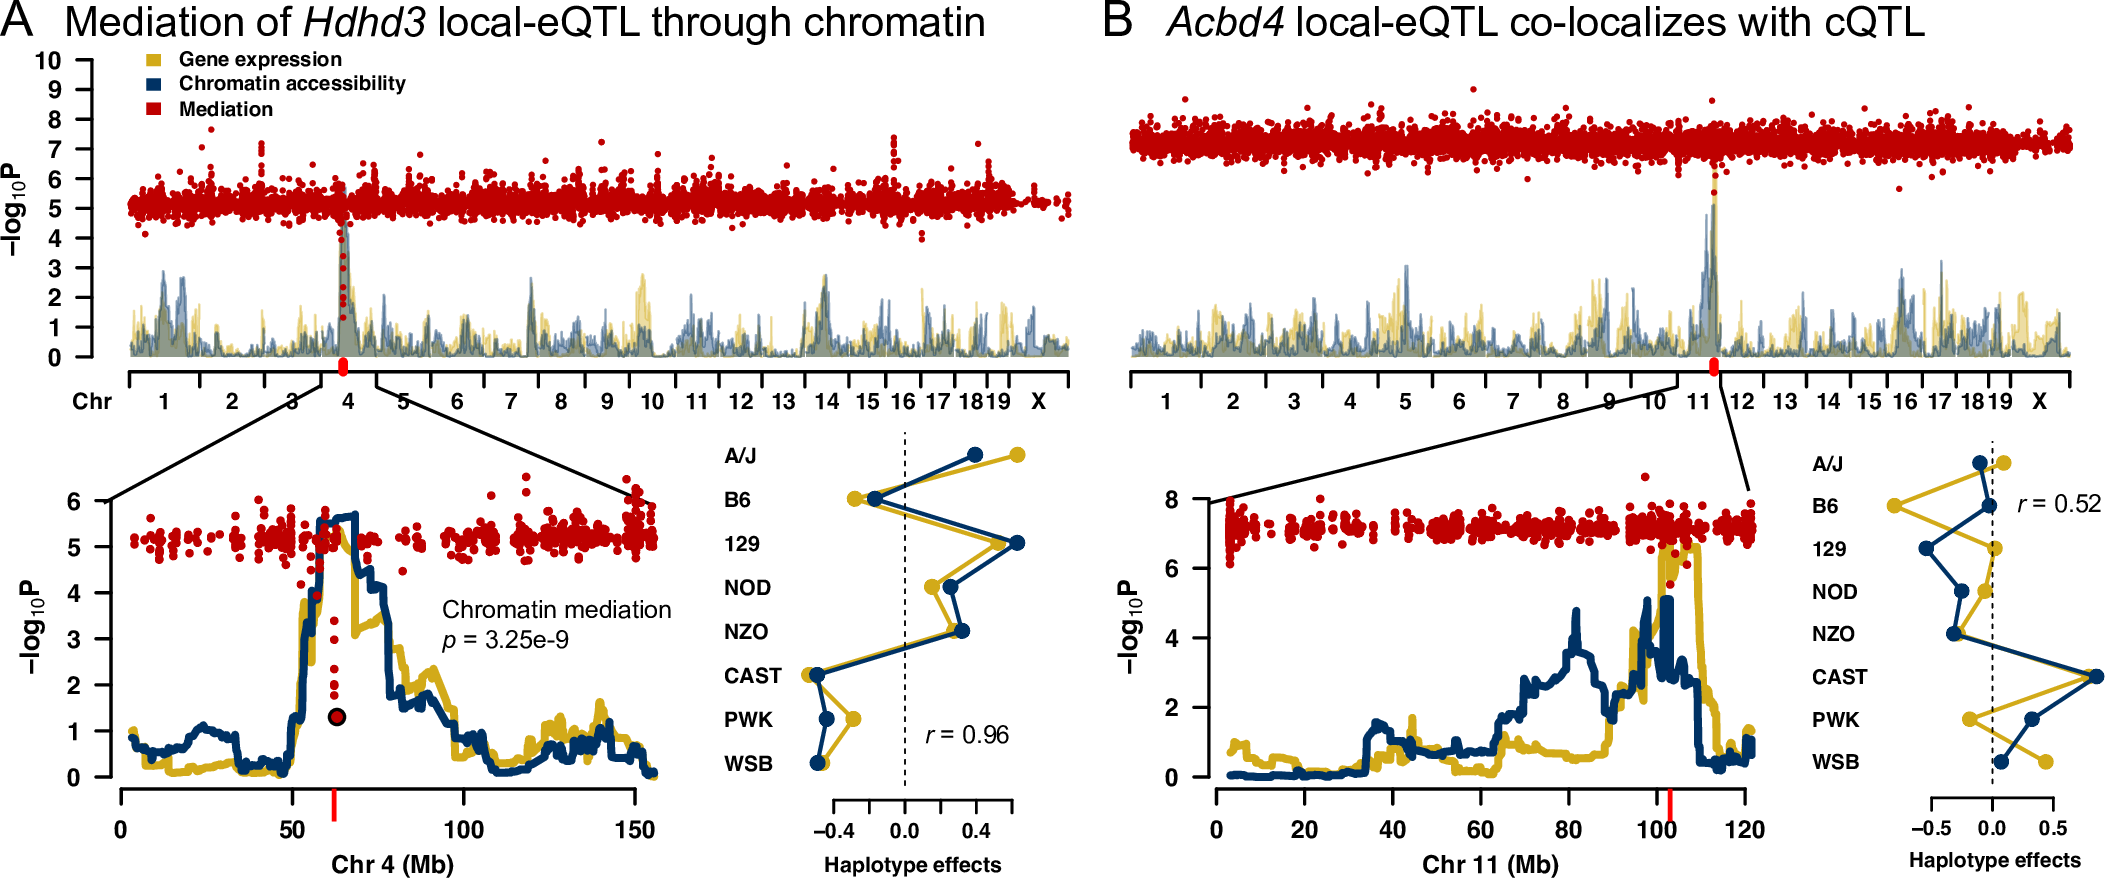
\includegraphics[width=\textwidth]{figs/mediation_or_colocal.png}
\caption{\textbf{Co-localizing eQTL and cQTL are not sufficient for statistical mediation.} 
The approach used to detect mediation through chromatin accessibility requires that the eQTL and cQTL co-localize (both within 10Mb of the gene TSS), as well as possess similar founder haplotype effect patterns. Co-localizing cQTL are observed for local-eQTL for both \textit{Hdhd3} in liver (A) and \textit{Acbd4} in kidney (B). QTL and mediation scans are shown, with chromosomes 4 and 11 blown up for \textit{Hdhd3} and \textit{Acbd4}, respectively. The red ticks denote the TSS for both genes. The founders effects were estimated as centered and scaled BLUPs. The founder effects for the eQTL and cQTL are highly correlated ($r = 0.96$) for \textit{Hdhd3}, but not for \textit{Acbd4} ($r = 0.52$). Strong mediation of the \textit{Hdhd3} eQTL through chromatin is detected, but not for \textit{Acbd4}. The effect size of the proximal cQTL to \textit{Acbd4} is smaller than its eQTL, also inconsistent with the relationship depicted in Fig 6A.
\label{fig:colocalization}}
\end{figure*}

\clearpage

\begin{figure*}[hp]
\renewcommand{\familydefault}{\sfdefault}\normalfont
\centering
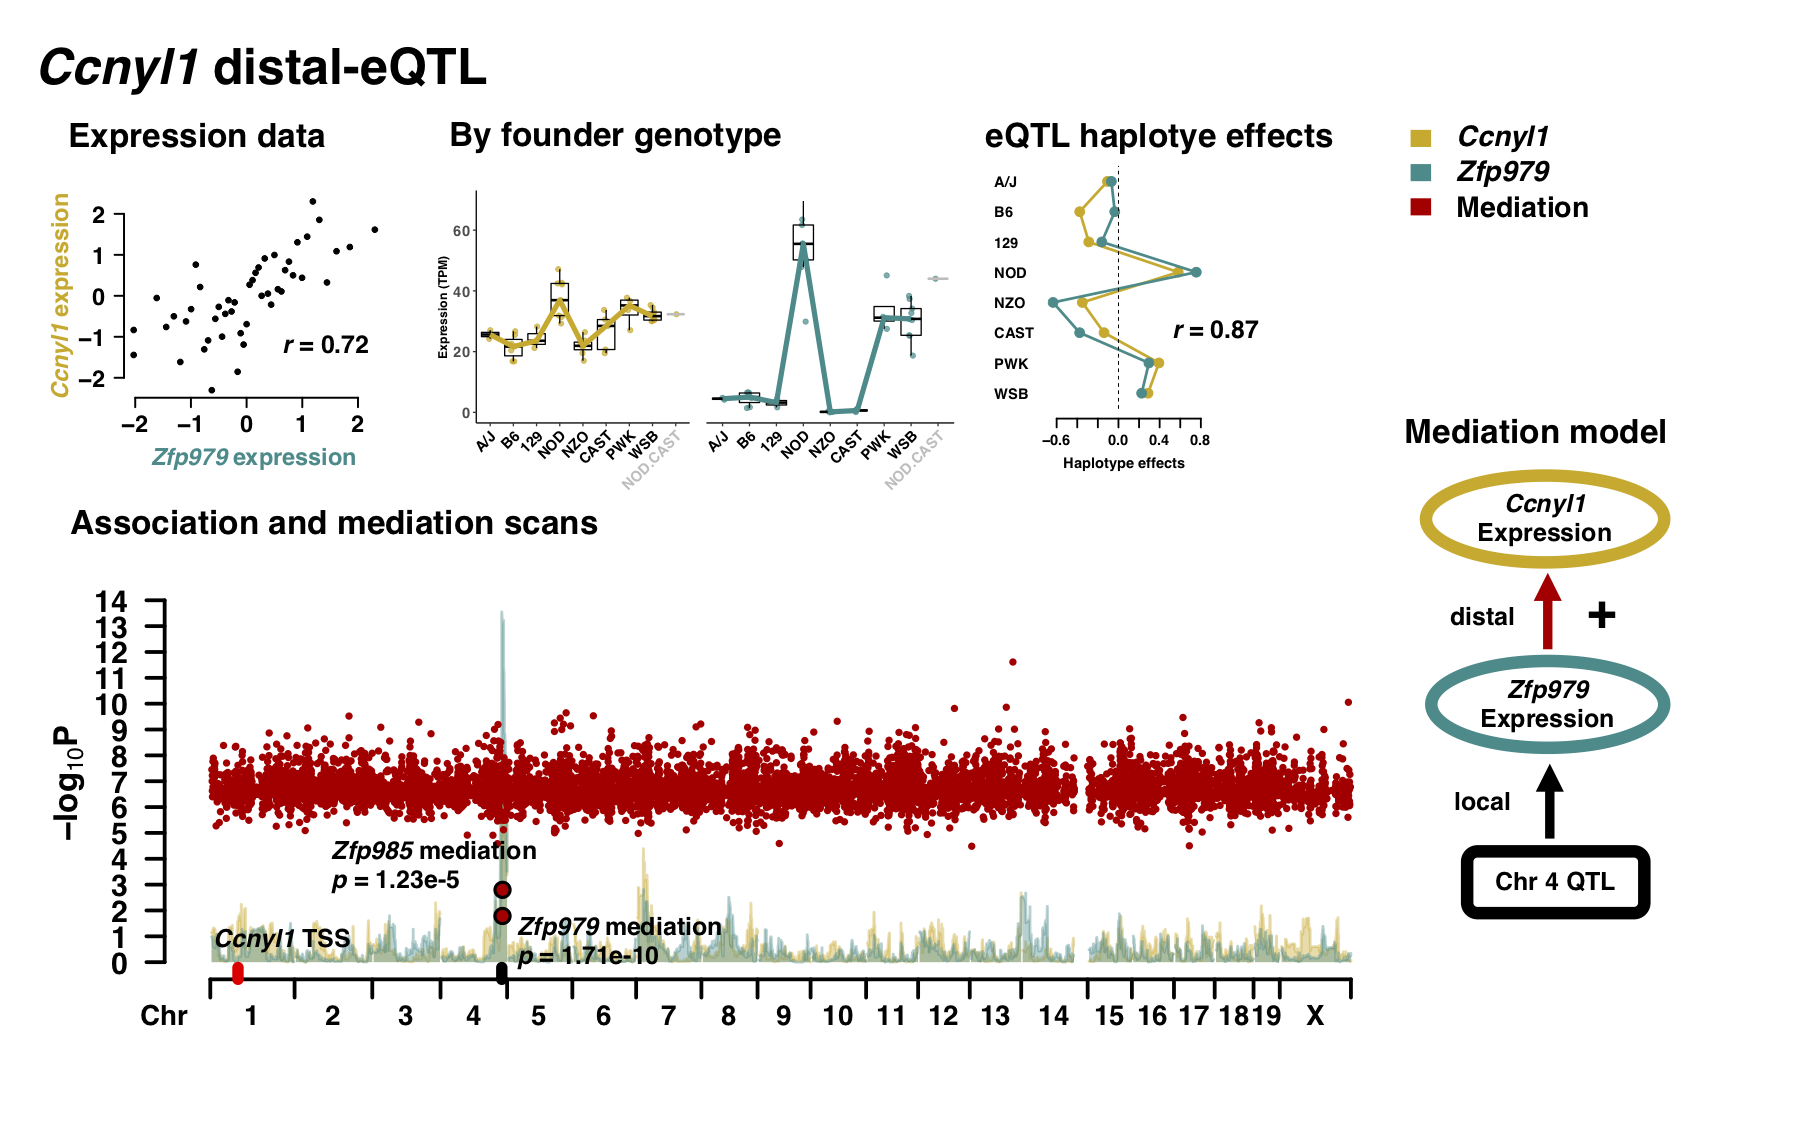
\includegraphics[width=\textwidth, trim={0in 0.5in 0in 0in}, clip]{figs/ccnyl1_mediation.png}
\caption{\textbf{Mediation of \textit{Ccnyl1} distal-eQTL through \textit{Zfp979} expression.} 
Expression of \textit{Ccnyl1} and \textit{Zfp979} are correlated ($r = 0.72$) in lung, which is also observed in the expression data categorized by diplotype and the founder effects estimated as scaled BLUPs. The distal-eQTL on chromosome 4 for \textit{Ccnyl1} corresponds closely to local-eQTL of \textit{Zfp979}. \textit{Ccnyl1} is located on chromosome 1, indicated by the red tick. \textit{Zfp979} and \textit{Zfp985}, both zinc finger proteins likely with DNA binding properties, are identified as strong candidate mediators of the distal-eQTL at genome-wide significance. The correlations, magnitude of effects, and mediation are consistent with the simple relationship depicted in the graph. The distal-eQTL and candidate mediators are located in a region of interest that regulates \textit{Akr1e1} expression. 
\label{fig:ccnyl1_exmediation}}
\end{figure*}

\clearpage

\begin{figure*}[hp]
\renewcommand{\familydefault}{\sfdefault}\normalfont
\centering
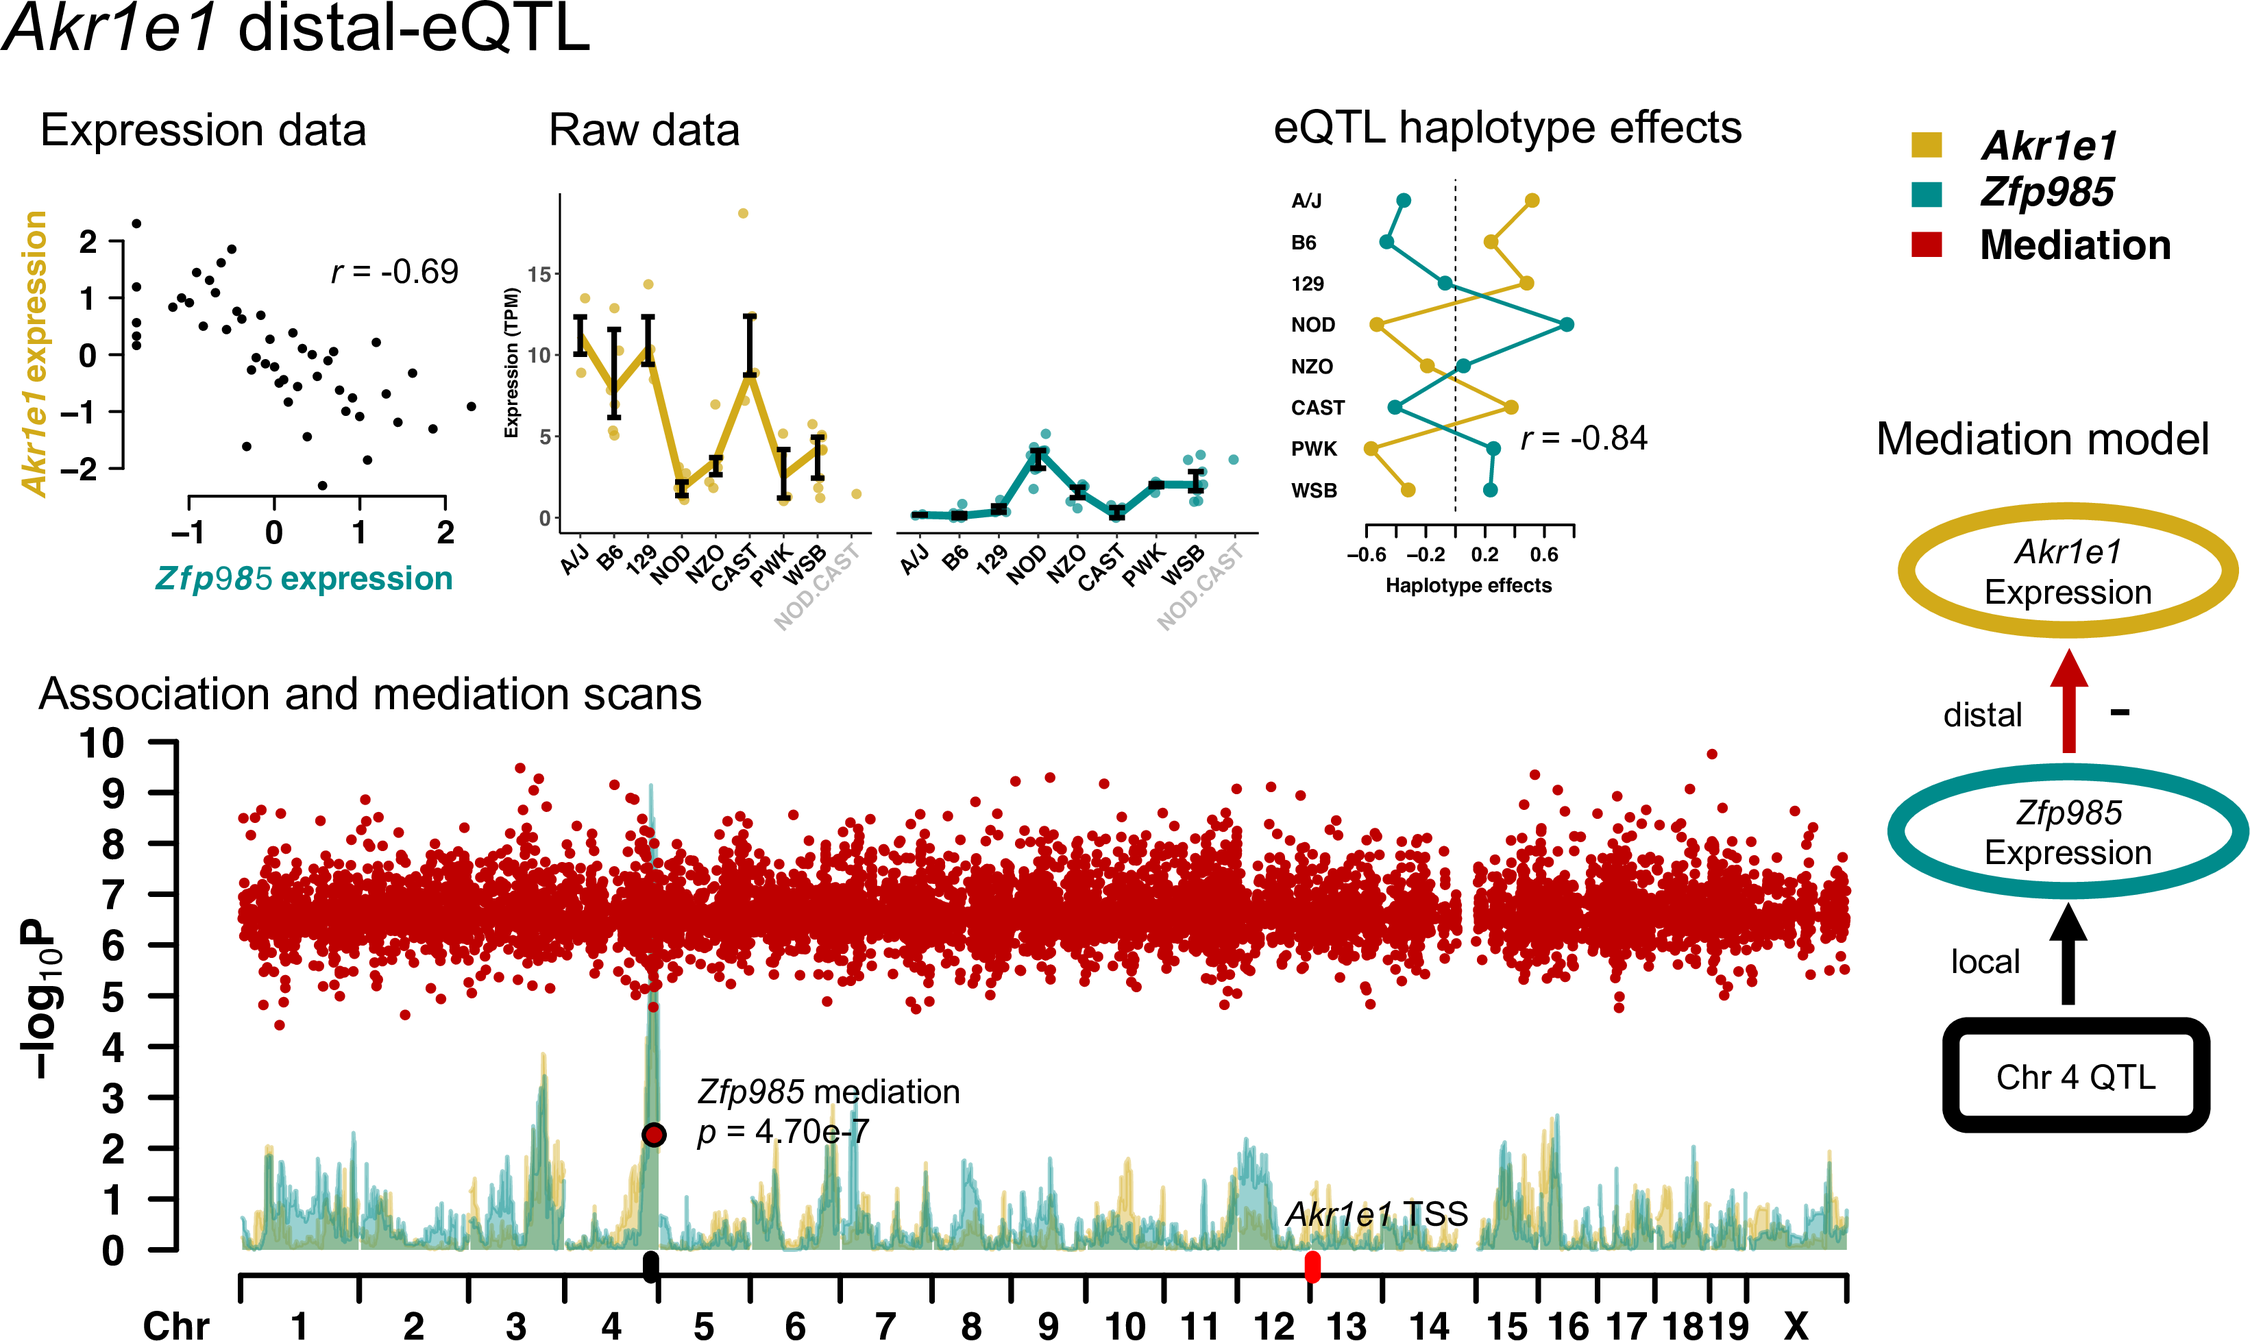
\includegraphics[width=\textwidth, trim={0in 0.5in 0in 0in}, clip]{figs/akr1e1_mediation.png}
\caption{\textbf{Mediation of \textit{Akr1e1} distal-eQTL through \textit{Zfp985} expression.} 
Expression of \textit{Akr1e1} and \textit{Zfp985} are anti-correlated ($r = -0.69$) in lung. This relationship is also observed in the expression data with bars representing the interquartile range, categorized by most likely diplotype, and the founder haplotype effects, estimated as scaled BLUPs. The QTL and mediation scans reveal that \textit{Akr1e1}, TSS marked with a red tick on chromosome 13, possesses a distal-eQTL on chromosome 4 that is proximal to the strong local-eQTL of \textit{Zfp985}. The mediation scan identifies \textit{Zfp985} as a strong candidate mediator consistent with the mediation model. A more complete picture of the genetic regulation of \textit{Akr1e1} expression is pieced together by looking across all three tissues and includes a potential chromatin mediator (Fig 9).
\label{fig:akr1e1_exmediation}}
\end{figure*}

\clearpage

\begin{figure*}[hp]
\renewcommand{\familydefault}{\sfdefault}\normalfont
\centering
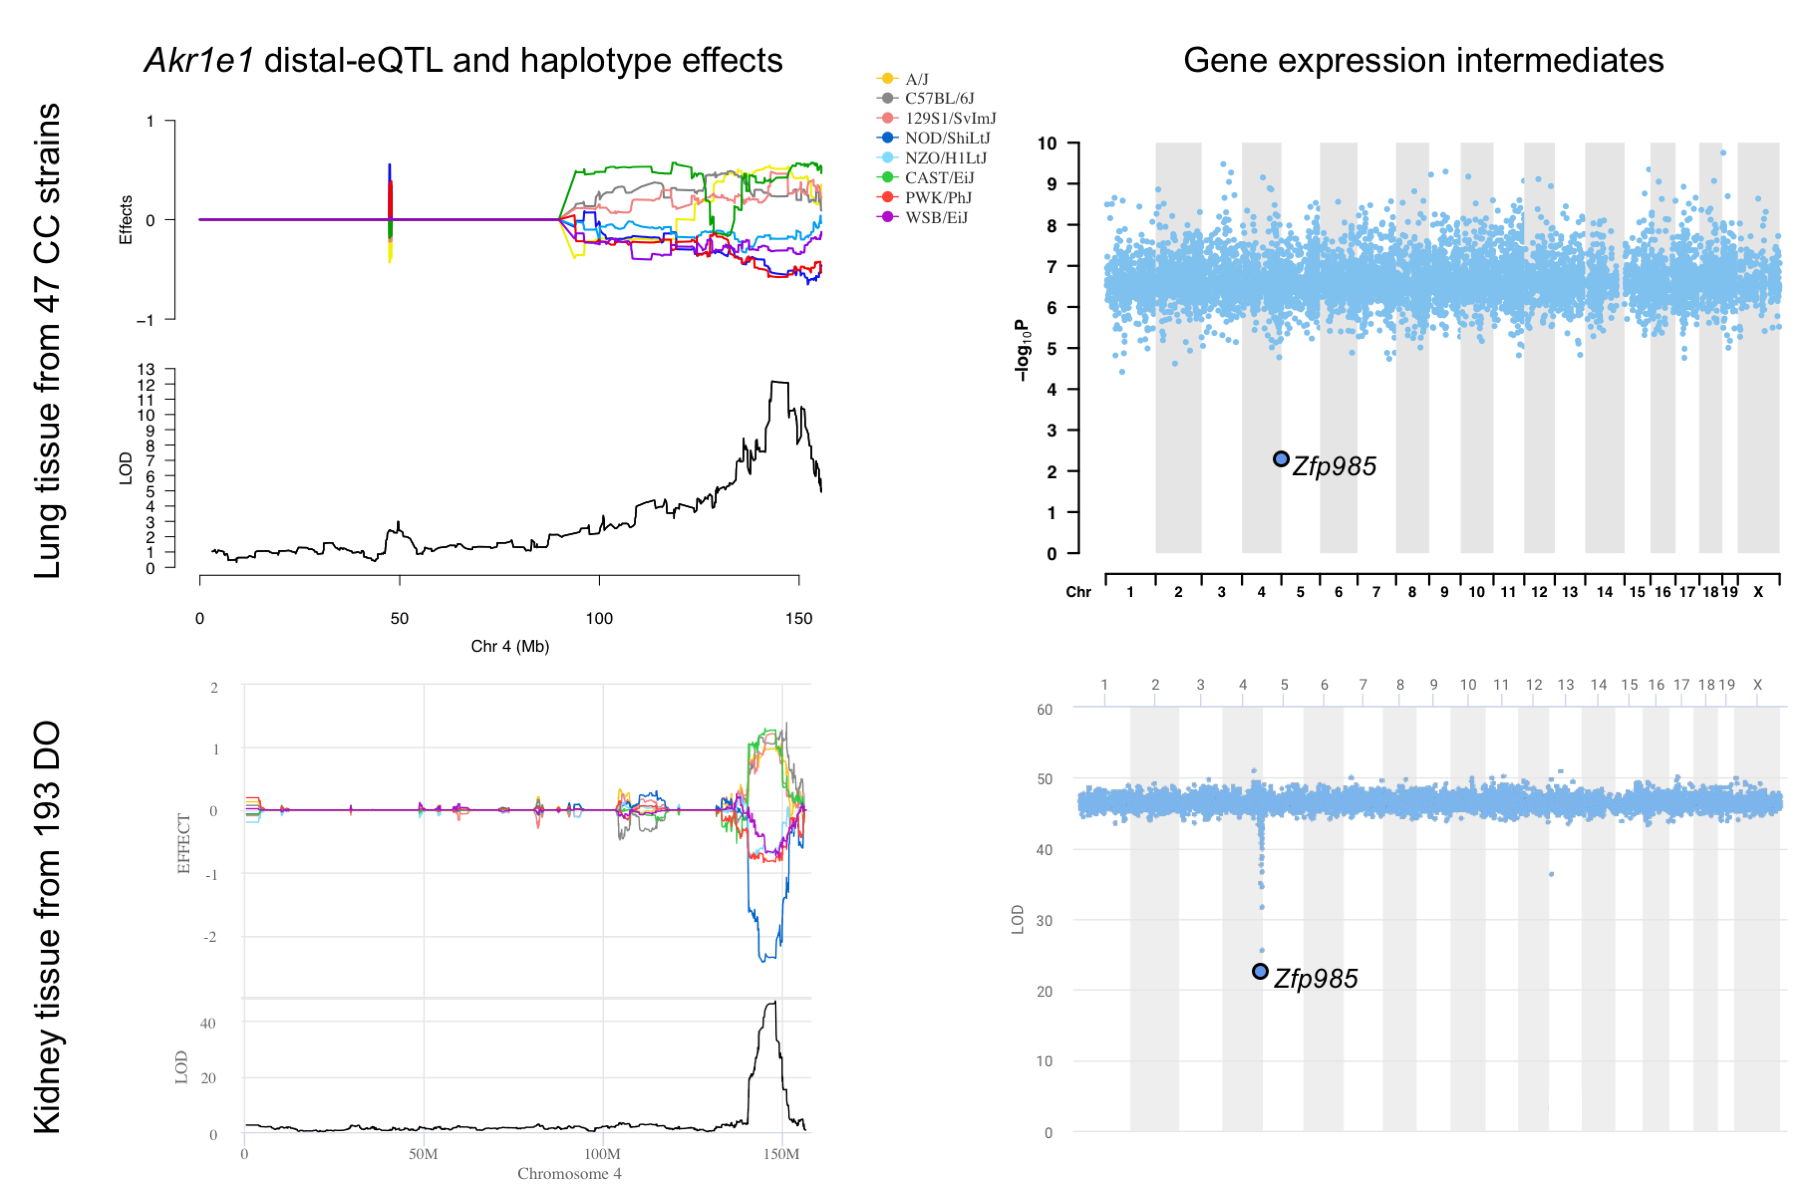
\includegraphics[width=\textwidth, trim={0in 0in 0in 0in}, clip]{figs/do_confirmation_akr1e1.png}
\caption{\textbf{Confirmation of \textit{Akr1e1} distal-eQTL and mediation by \textit{Zfp985} in kidney tissue of Diversity Outbred mice.} 
A genome-wide significant distal-eQTL was detected for \textit{Akr1e1} in liver, lung (shown here), and kidney tissues from 47 CC strains. In a larger sample of kidney tissue from outbred DO mice, the same distal-eQTL and mediation relationship were observed. As expected, the larger sample results in greater statistical significance, and confirms that the NOD effect is more strongly negative than NZO, PWK, and WSB, which the effects plots the \textit{Zfp985} local-eQTL suggested. Notably, \textit{Zfp985} was not tested in the CC kidney because of low levels, though the distal-eQTL for \textit{Akr1e1} is consistent with its activity, which is here confirmed in the DO.
\label{fig:do_akr1e1}}
\end{figure*}

\clearpage

\begin{figure*}[hp]
\renewcommand{\familydefault}{\sfdefault}\normalfont
\centering
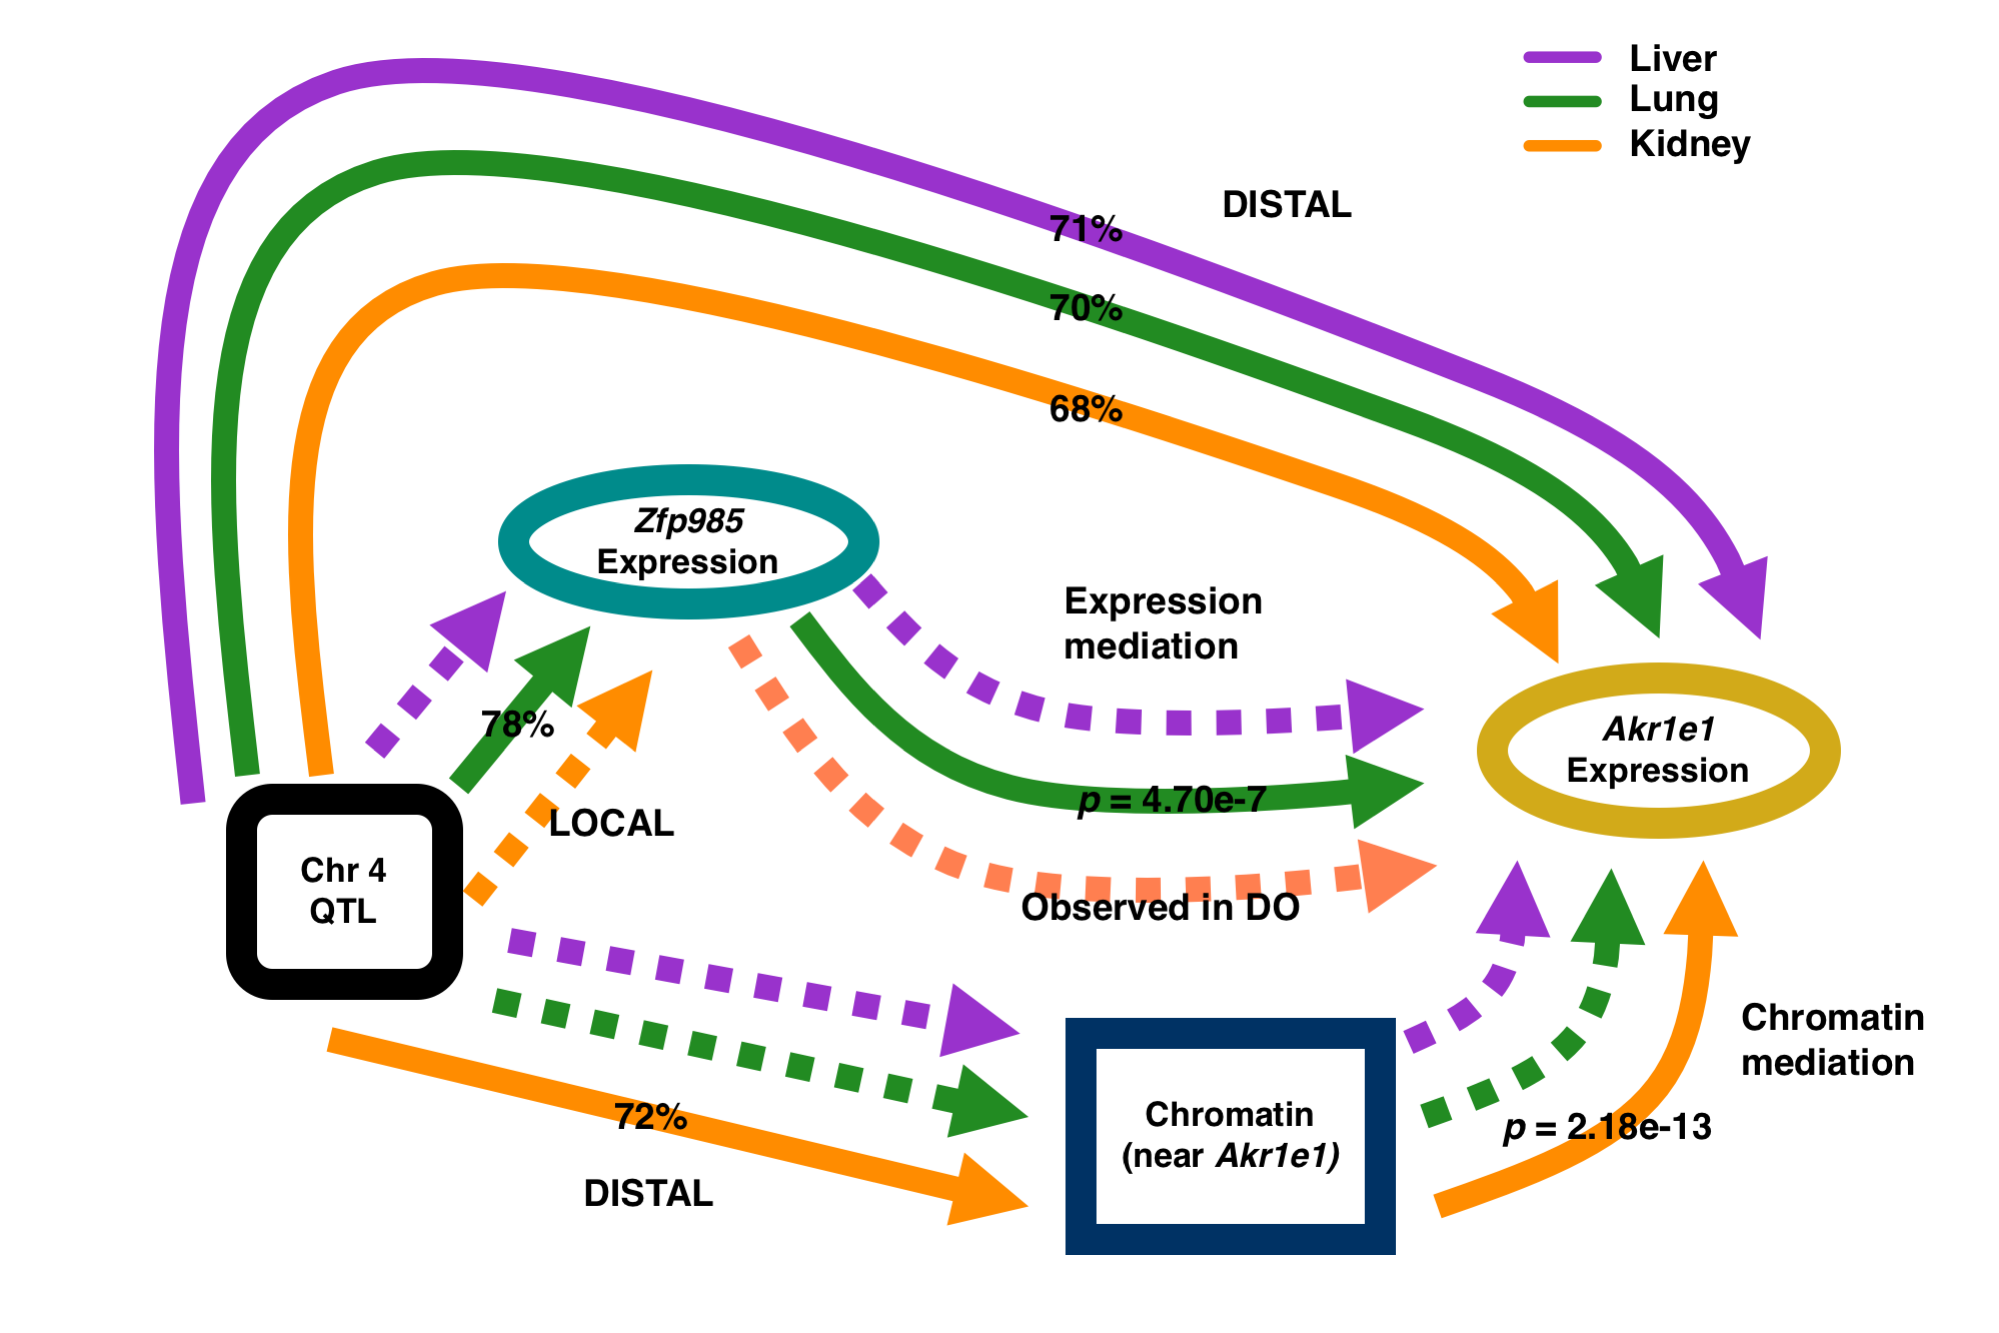
\includegraphics[width=\textwidth, trim={0in 0in 0in 0in}, clip]{figs/akr1e1_observed_relationships.png}
\caption{\textbf{Observed relationships across the three tissues related to the genetic regulation of \textit{Akr1e1} expression.} 
The model for the distal genetic regulation of \textit{Akr1e1} expression, described in Figure \ref{fig:akr1e1_full_model}, was reconstructed from these observed relationships. Solid arrows were observed, whereas dashed arrows are assumed. Effect sizes represent the proportion of variance explained by the QTL and mediation $p$-values (permP) were defined using a permutation procedure. The assumed relationships are supported by the presence of the distal-eQTL in all three tissues. The \textit{Zfp985} mediator relationship in kidney, though not observed in the CC, was observed in the related DO population.
\label{fig:akr1e1_relationships}}
\end{figure*}

\clearpage

\begin{figure*}[hp]
\renewcommand{\familydefault}{\sfdefault}\normalfont
\centering
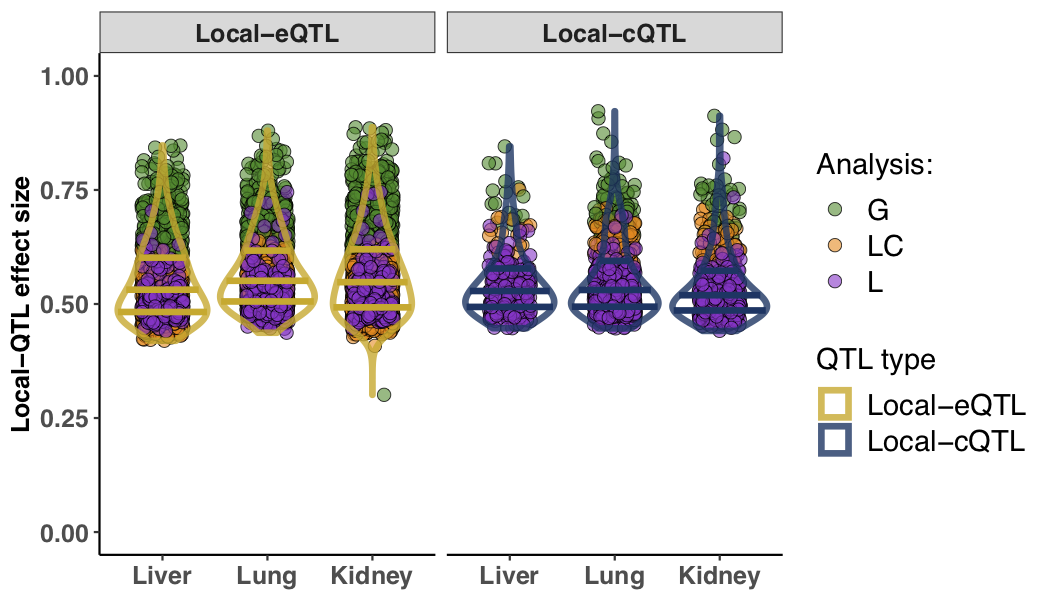
\includegraphics[width=\textwidth, trim={0in 0in 0in 0in}, clip]{figs/local_qtl_effects.png}
\caption{\textbf{Local-QTL effect sizes by mapping analysis.} Based on ranking mapping analyses with respect to the extent of scope, local (L; magenta) to chromosome (C; plum) to genome-wide (G; cyan), the greater the scope corresponded to reduced power to detect QTL, shown in liver, lung, and kidney tissues for gene expression (yellow line) and chromatin accessibility (blue line). Each dot represents a detected local-QTL, colored according to the highest scope mapping procedure that detected it. The three horizontal bars represent the 25\textsuperscript{th}, 50\textsuperscript{th}, and 75\textsuperscript{th} quantiles of QTL effect sizes for all local-QTL per tissue. Analysis G generally detects QTL with effect size $>$ 60\%, whereas Analyses C and L detect QTL effect sizes $>$ 45\%. Effect size estimates correspond to a fixed effects model of the QTL.
\label{fig:qtl_effect_sizes_by_method}}
\end{figure*}

\clearpage

\begin{figure*}[hp]
\renewcommand{\familydefault}{\sfdefault}\normalfont
\centering
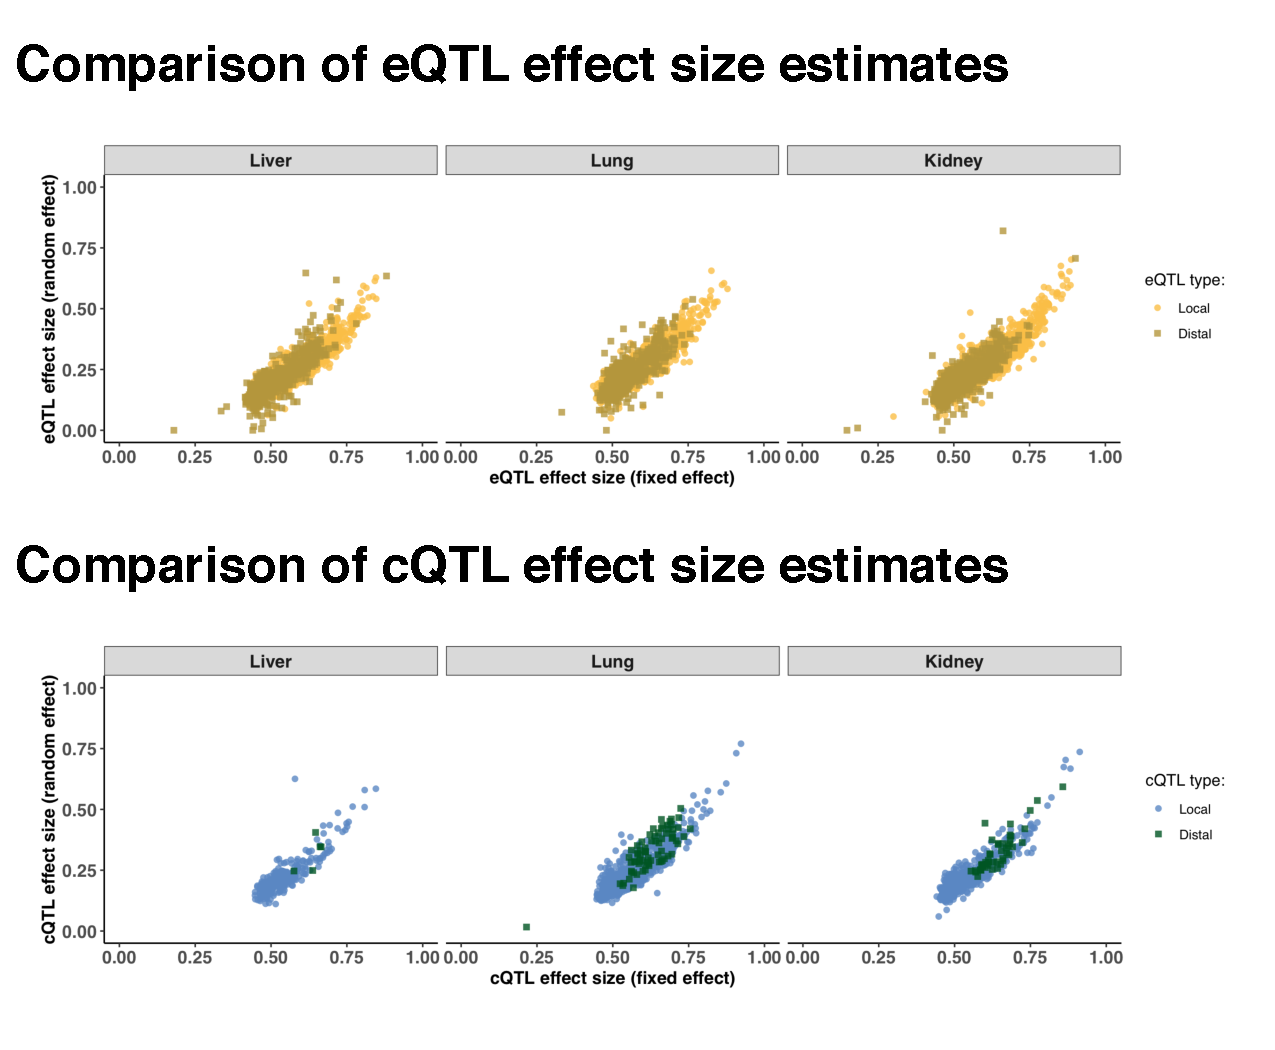
\includegraphics[width=0.9\textwidth, trim={0in 0in 0in 0in}, clip]{figs/fixefvsranef_qtl.pdf}
\caption{\textbf{Comparison of QTL effect sizes estimates from fixed effects and random effects models.} 
The effect size corresponding to the random effect fit is harshly penalized compared to the fixed effect estimate, likely due to a modest sample size of 47 individuals. Notably, there are a number of distal-eQTL that are more harshly reduced by the random effects model compared to the other QTL, likely representing signals resulting from extreme observations or imbalances in founder contributions at the locus. QTL detected by Analyses G (FDR $< 0.1$), C (FDR $< 0.1$), and L are shown.
\label{fig:qtl_effect_size_fixefvsranef}}
\end{figure*}

\begin{figure*}[hp]
\renewcommand{\familydefault}{\sfdefault}\normalfont
\centering
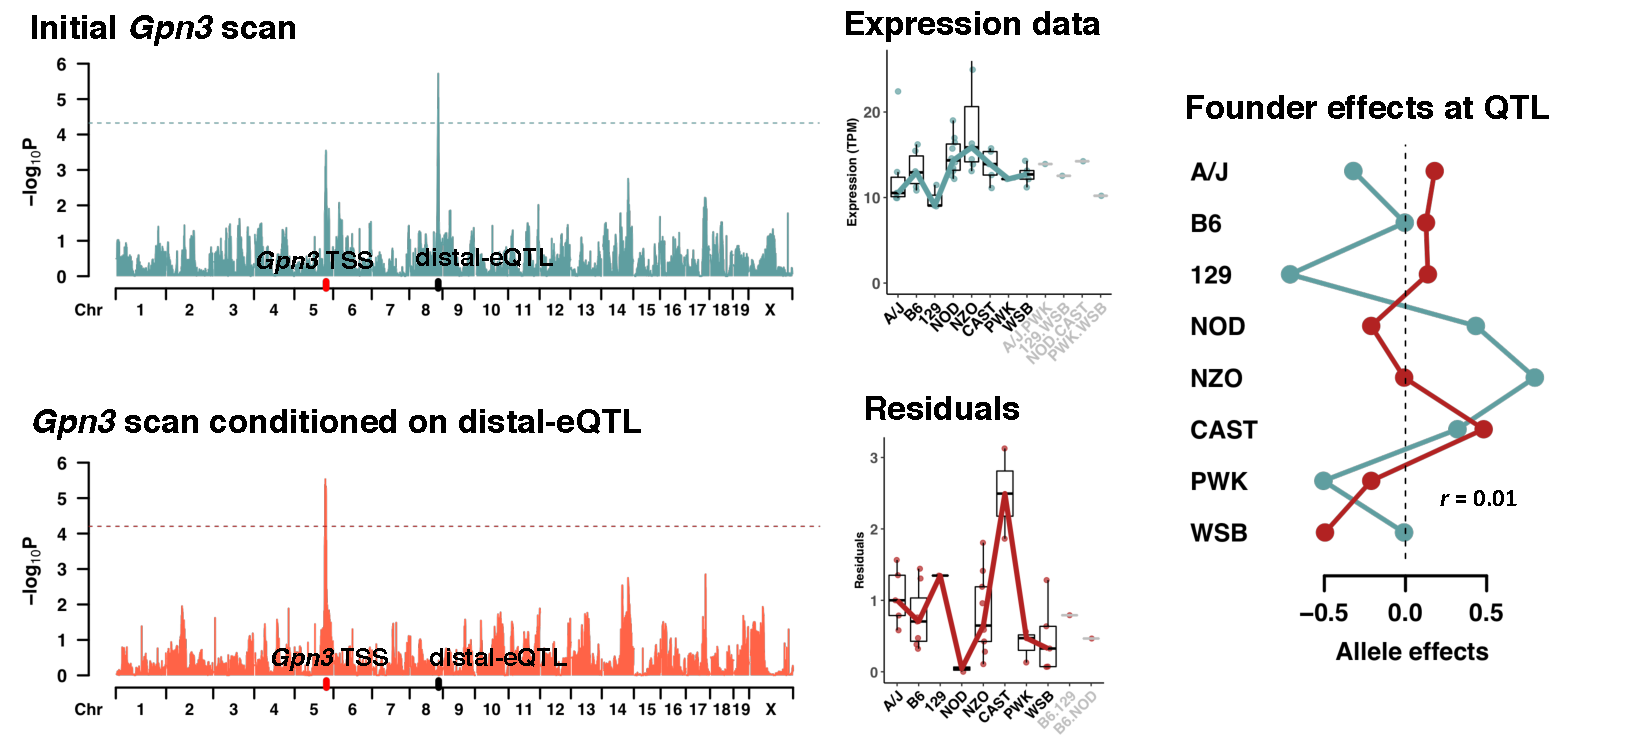
\includegraphics[width=\textwidth, trim={0in 0in 0in 0in}, clip]{figs/gpn3_conditional_scan.pdf}
\caption{\textbf{Detection of local-eQTL after conditioning on distal-eQTL for \textit{Gpn3}.} 
The multi-stage conditional regression approach of Analysis G allows for the detection of multiple genome-wide significant QTL, which can then be appropriately incorporated into a FDR procedure across many outcomes. In this example in lung tissue, the gene \textit{Gpn3} initially has a strong distal-eQTL on chromosome 8 (A). Though a peak is detected near the TSS of \textit{Gpn3}, it does not meet genome-wide significance. However, after conditioning on the distal-eQTL, the local-eQTL is detected (B). Horizontal dashed lines represent empirical 95\% significance thresholds based on 1,000 permutations.
\label{fig:conditional_scans}}
\end{figure*}


\end{document}


